\documentclass[sig-alternate]{article}  
\usepackage{ltexpprt}
\usepackage{pst-3dplot}
\usepackage{subfigure}
\usepackage{algorithm}
\usepackage{algorithmicx}
\usepackage[noend]{algpseudocode}
\usepackage{graphics}
\usepackage{graphicx}
\usepackage{epsfig}
\usepackage{amsmath}
\usepackage{amssymb}
\usepackage{float}
\usepackage{fancybox}
\usepackage{url}
\usepackage{wrapfig}
\usepackage{cite}
\usepackage{times}
\usepackage[english]{babel}
\usepackage{units}
\usepackage[normalem]{ulem}

\pagestyle{empty}
\thispagestyle{plain}

\begin{document}

\title{Economically-Efficient Sentiment Stream Analysis}

\numberofauthors{6} %  in this sample file, there are a *total*
% of EIGHT authors. SIX appear on the 'first-page' (for formatting
% reasons) and the remaining two appear in the \additionalauthors section.
%
\author{
% You can go ahead and credit any number of authors here,
% e.g. one 'row of three' or two rows (consisting of one row of three
% and a second row of one, two or three).
%
% The command \alignauthor (no curly braces needed) should
% precede each author name, affiliation/snail-mail address and
% e-mail address. Additionally, tag each line of
% affiliation/address with \affaddr, and tag the
% e-mail address with \email.
%
% 1st. author
\alignauthor
Ben Trovato\titlenote{Roberto Oliveira Júnior}\\
       \affaddr{Computer Science Dept, Federal University of Minas Gerais\titlenote{The Ohio State University}\\
       \email{robertolojr@dcc.ufmg.br}
% 2nd. author
\alignauthor
Adriano Veloso}\\
       \affaddr{Computer Science Dept, Federal University of Minas Gerais}\\
       \email{adrianov@dcc.ufmg.br}
% 3rd. author
% 2nd. author
\and
\alignauthor
Adriano Pereira}\\
       \affaddr{Computer Science Dept, Federal University of Minas Gerais}\\
       \email{adrianoc@dcc.ufmg.br}
\and  % use '\and' if you need 'another row' of author names
% 4th. author
\alignauthor
Wagner Meira Jr}\\
       \affaddr{Computer Science Dept, Federal University of Minas Gerais}\\
       \email{meira@dcc.ufmg.br}
% 5th. author
\and
\alignauthor
Renato Ferreira}\\
       \affaddr{Computer Science Dept, Federal University of Minas Gerais}\\
       \email{renato@dcc.ufmg.br}
% 6th. author
\and
\alignauthor Srinivasan Parthasarathy\\
       \affaddr{Dept. of Computer Science and Engineering and Department of Biomedical Informatics\\The Ohio-State University\\}\\
       \email{srini@cse.ohio-state.edu}
}
% 
% \author{
% Roberto Louren\c{c}o$^{a,b}$ \and Adriano Veloso$^a$ \and Adriano Pereira$^a$ \and Wagner Meira Jr.$^a$ \and Renato Ferreira$^a$ and Srinivasan Parthasarathy$^b$\\\\
% $^a$ Computer Science Dept, Federal University of Minas Gerais\\
% \{robertolojr,adrianov,adrianoc,meira,renato\}@dcc.ufmg.br\\
% $^b$ Dept. of Computer Science and Engineering and Department of Biomedical Informatics\\The Ohio-State University\\
% srini@cse.ohio-state.edu
% }
\date{}
\maketitle

\vspace{-0.2in}

\begin{abstract}
Text-based social media channels, such as Twitter, produce
torrents of opinionated data about the most diverse topics and entities.
The analysis of such data (aka. sentiment analysis) is quickly becoming a key feature in recommender systems
and search engines.
A prominent approach to sentiment analysis is based on the application of classification techniques, that is,
content is classified according to
the attitude of the writer.
A major challenge, however, is that Twitter
follows the data stream model, and thus classifiers must operate
with limited resources, including labeled data and time for building classification models. Also challenging is the fact that
sentiment distribution may change as the stream evolves.
In this paper we address these challenges by proposing algorithms that separate relevant training instances at each time step, so that training windows are kept small while providing to the classifier the capabilities to suit itself to, and to recover itself from, sentiment drifts. Simultaneously providing both capabilities to the classifier, however, is
a conflicting-objective problem, and our algorithms employ notions of Economics in order to balance both capabilities. We performed the analysis of events that reverberated on Twitter,
and the comparison against the state-of-the-art reveals improvements in terms of error reduction (up to 14\%) and reduction of training resources (by orders of magnitude).
\end{abstract}

\section{Introduction}

The need for real-time text analytics is clear and present given the ubiquitous reach of social media sites like Facebook and Twitter. Specifically, recognizing customer sentiment in real-time and enabling advertising on-the-fly have the potential to be a breakthrough technology~\cite{forbes}.
%(\url{http://www.forbes.com/sites/lorikozlowski/2012/04/24/twitter-and-our-feelings-real-time-sentiment-analysis}).
Early examples of such technology in use were demonstrated in this year's National Football League's Superbowl (a premier sporting event in the USA) where a well known manufacturer of {\em Oreo} cookies took advantage of a third quarter blackout (and associated Twitter sentiment) to embed a contextual advertisement. Another example at the same event was the advertisement for a Hollywood movie, where, based on the initial advertisement which happened before the start of the first quarter (and associated Twitter sentiment), the decision on which of several possible advertisements to run later on in the program was apparently taken as a runtime decision.
Examples like these are likely to occur more frequently due to
%Examples such as these are likely to occur more frequently in the near future, going beyond advertising.
lightweight and easy communication mechanisms, such as Twitter microblogging, which makes people eager not only to exchange information, but also to convey their opinions and emotions. People watch events together on television, while tweeting out about things happening around them. As a result, opinionated content is created almost at the same time the event is happening in the real world, and becomes available shortly after.  The analysis of such content (aka. sentiment analysis) in order to exploit the aggregate sentiment of the online crowd goes beyond advertising, and is becoming crucial to recommender systems and search engines.

There is a growing trend in performing sentiment analysis using classification-related techniques: a process that automatically
builds a classification model by learning, from a set of previously
labeled data (i.e., the training-set), the underlying characteristics that distinguish one sentiment from another (i.e., happiness, madness, surprise, suspicion). The success of these classifiers
rests on their ability to judge attitude by means of textual-patterns present in the data, which usually appear in the form
of (idiomatic) expressions and combinations of words.
Sentiment analysis over Twitter real-time messages, however, is particularly challenging, because: (i) Twitter follows the data stream model\footnote{
There are three main source streams in Twitter. The Firehose provides all status updates from everyone in real-time.
Spritzer and Gardenhose are two sub-samples of the Firehose. The current sampling rates are 5\% and 15\%, respectively.},
requiring classifiers to operate with limited computing and training resources, 
%(ii) the training-set is potentially noisy, since training messages may be (incorrectly) labeled using either author-provided sentiment indicators (i.e., emoticons and hash tags~\cite{sigir,tags}) or via crowdsourcing annotation,
and (ii)
either sentiment distribution or the characteristics related to certain sentiments may change over time in almost unforeseen ways (i.e., sentiment drift).

%\paragraph*{\bf{Our Approach to Sentiment Stream Analysis}}
\subsection*{Our Approach to Sentiment Stream Analysis}
A possible strategy to cope with the aforementioned challenges is to employ selective sampling algorithms in order to
focus only on the most relevant training examples/messages at
each time step and to creating training sets from which classifiers are built. Such
training sets are kept as small as possible to ensure fast learning times, since a new classifier must be built at each time step, after a new target message arrives.
Also, messages should be
selected so that the resulting training set
provides sufficient resources to enable the resulting classifier to be effective under the occurrence of drifts.
In order to provide sufficient training resources while keeping sets small, our algorithms select training messages by taking into account two
important properties, that we define as adaptiveness and memorability.
Informally, adaptiveness enables the classifier to adapt
itself to drifts, and thus, improving adaptiveness involves incorporating fresh messages into
the current training set, while discarding obsolete ones. Memorability, on the other hand, involves retaining messages belonging to pre-drift distributions,
therefore enabling the classifier to recover itself from drifts.

We hypothesize that adaptiveness and memorability are both necessary to make classifiers robust to drifts. 
However, given their antagonistic natures, improving both properties may lead to a conflicting-objective problem, in which the attempt to improve memorability further may result in worsening adaptiveness.
Thus, we tackle the problem
by proposing selective sampling algorithms based on multi-objective optimization, that is, we propose to select training messages so that the resulting classifier achieves a proper balance between memorability and adaptiveness.
Our algorithms are based on
central concepts in Economics, namely {\em Pareto} and {\em Kaldor-Hicks} efficiency criteria~\cite{palda@book,kaldor,hicks}. The Pareto Efficiency criterion informally states
that ``when some action could be done to make someone better off without
hurting anyone else, then it should be done.'' This action is called Pareto improvement,
and a system is said to be Pareto-Efficient if no such improvement is possible.
The Kaldor-Hicks criterion is less stringent and states that ``when some action could be done to make someone better off, and this could compensate those that are made worse off, then it should be done.''

\subsection*{Contributions and Findings}
%\paragraph*{\bf{Contributions and Findings}}
The main contribution of this paper is to exploit the intuition behind the aforementioned concepts for devising new algorithms for sentiment stream analysis.
In practice, we claim the following benefits and contributions:


\begin{itemize}
\item We formulate simple-to-compute yet effective utility measures that capture the notions of adaptiveness and memorability. For instance, the similarity between messages that are candidate to compose the current training set and the target message, as well as the freshness of the candidate messages, are measures that tend to privilege adaptiveness. In contrast, candidate messages are also randomly shuffled, thus privileging memorability. These utility measures result in a utility space, and the extent to which each candidate message contributes to adaptiveness and memorability depends on where it is placed in this space.
\item We exploit the concept of Pareto Efficiency by separating messages (viewed as points in the utility space) that are not dominated by any other message. These messages compose the Pareto frontier~\cite{palda@book}, and messages lying in this frontier correspond to cases for which no Pareto improvement is possible. These messages privilege either adaptiveness or memorability, and thus they are selected to compose the current training set from which the classifier is built.
\item We exploit the concept of Kaldor-Hicks Efficiency by selecting an additional set of messages that, although not lying in the Pareto frontier, correspond to a positive trade-off between adaptiveness and memorability. These messages are selected to compose the current training set from which the classifier is built.
\item Our algorithms may operate either on an instance-basis or in batch-mode, by employing classification models based on sentiment rules that are kept incrementally as the stream evolves and training sets are modified.
\end{itemize}

%While every Pareto improvement is a Kaldor-Hicks improvement, most Kaldor-Hicks improvements are not Pareto improvements. That is, the set of Pareto improvements is a proper subset of Kaldor-Hicks improvements, which reflects the greater flexibility and applicability of the Kaldor-Hicks criterion relative to the Pareto criterion.

%We exploit these efficiency concepts as follows. Each possible training message is associated with a point in an n-dimensional scattergram (which we call utility space). In this case, a point is represented as $[a_1, a_2, \ldots, a_n]$, where each coordinate $a_i$ corresponds to a quantity that is either related to adaptiveness or memorability.
%Points that are not dominated by any other point in the scattergram compose the Pareto frontier~\cite{palda@book}. Points lying in the frontier correspond to cases for which no Pareto improvement is possible, being therefore messages likely to privilege either adaptiveness or memorability at a particular time step. Dominated messages are discarded, while messages in the frontier are selected to compose the current training set, from which the classifier is built. 
%A broader frontier, composed of additional training messages, can be built using the Kaldor-Hicks criterion. The process of building the classifier from the messages in the (either Pareto or Kaldor-Hicks) frontier is repeated every time a new target message arrives in the stream.

To evaluate the effectiveness of our algorithms, we
performed experiments using Twitter data collected from three important events in 2010, spanning different sentiments expressed in different languages.
Results show that our algorithms make classifiers extremely effective, with gains in prediction performance that are up to 14\% when compared against the state-of-the-art. Further, the amount of training resources needed is decreased by two orders of magnitude.

\section{Related Work}

In the data stream model, data arrives at high speed and algorithms must
work in real time and with limited resources. Further, in some domains,
algorithms must deal either with burst detection~\cite{shasha} and concept drift (i.e.,
data which nature or distribution change over time). \v{Z}liobait\.{e}
\cite{DBLP:journals/corr/abs-1010-4784} categorizes such drifts as sudden, gradual,
incremental and recurring. When data distribution or nature change over time, its relevance
must be recalculated to avoid harming the model. This kind of data stream is known as
evolving data streams.

Many techniques have been proposed to allow accurate classification in evolving data
streams.  N\'{u}\~{n}ez et al. \cite{Nunez:2007:LEU:1314498.1390328} proposed a
method for keeping a variable training window by adjusting internal
structures of decision trees. An ensemble of Hoeffding trees have been proposed
in \cite{Bifet:2012:ERH:2089094.2089106}, each tree is limited to a small subset of
attributes. Gama et al.\cite{Gama2009a} proposed a mechanism to discard old
information based on sliding windows. Bifet et al.  \cite{Bifet2007,
Bifet:2009:ALE:1617420.1617445} proposed an adaptive sliding window algorithm,
called ADWIN, suitable for data streams with sudden drifts.
The approach presented in
\cite{Koychev00gradualforgetting} suggests that a time-based
forgetting function, which makes more recent observations more significant,
provides adaptiveness to the classifier.
Klinkenberg \cite{Klinkenberg:2004:LDC:1293831.1293836} compares example selection, often
used in windowing approaches with example weights. Experiments
show that both approaches are effective.
In \cite{sigir} the
authors proposed an approach based on a training augmentation procedure, which
automatically incorporates
relevant training messages into the training-set.
%Classification models are produced
%on-the-fly using association rules, which are kept up-to-date in an incremental
%fashion, so that at any given time the model properly reflects the sentiments
%in the event being analyzed.

Some works have focused on feature similarity, such as Torres et al.
\cite{Torres:2011:CMD:2025756.2025758} that studied different methods for data
stream classification and proposed a new way of keeping the representative
data models based on similarity measures.
Feng et al. \cite{Feng2013} extracted the
concept from each data block using feature similarity
probabilities. 
Masud et al. \cite{Masud:2008:PAC:1510528.1511337} proposed a novel technique
to overcome the lack of labeled examples by building models
from unlabeled instances and a small amount of labeled ones.
Zhu et al. \cite{5440901} employed active learning to produce a
classifier ensemble that selects labeled instances from data streams to
build classifiers. Also, in \cite{6414645,Indre2011k} active
learning approaches are presented for data streams that explicitly handle
concept drifts. They are based on uncertainty~\cite{uncertainty}, dynamic allocation 
of labeling efforts over time, and randomization of the search space. \v{Z}liobait\.{e} et
al.  \cite{DBLP:journals/jmlr/ZliobaiteBHP11} proposed a system that implements active
learning strategies, extending the Massive Online Analysis (MOA) framework \cite{moa}.

Works above cited attempt to face concept drift in data stream through manipulation of
classifiers, with mechanisms such as training windows and decay functions,
active learning and sampling. In this paper we present new algorithms that
select high-utility examples in order to provide adaptiveness and memorability
to the classifier. In order to balance adaptiveness
and memorability, we formalized this issue as a multi-objective problem. The sample
selection is performed using economic efficiency criteria: Pareto and Kaldor-Hicks.
%Also, we discuss algorithms that operate under instance-basis and batch-mode scenarios. In particular, the batch-mode scenario enables our algorithms to
%reduce labeling effort.
We did not find in the recent literature
approaches that employ multi-objective models based on economic efficiency criteria to
deal with issues in the data stream environment.

\section{Algorithms}

In this section we present novel selective sampling approaches for learning classifiers to distinguish between different sentiments expressed in Twitter messages. We start by discussing models based on specialized association rules.
Then we present measures for adaptiveness and memorability, and describe the message utility space. Finally, we discuss Pareto and Kaldor-Hicks criteria, and algorithms that select training messages using these criteria.

\subsection{Sentiment Stream Analysis}

In our context, the task of learning sentiment streams is precisely defined as follows. At time step $n$, we have as input
a training set referred to as $\mathcal{D}_n$, which consists of
a set of records of the form $<d,s_i>$, where $d$ is a
message (represented as a list of terms),
and $s_i$ is the sentiment implicit in $d$.
The sentiment variable $s$ draws its values from a pre-defined, fixed and discrete set of possibilities (e.g., $s_1$,
$s_2$, $\ldots$, $s_k$).
The training set is used to build a classifier relating textual patterns in the messages to their corresponding sentiments.
A sequence of future messages referred to as $\mathcal{T}=\{t_n, t_{n+1}, \ldots\}$, consists of messages
for which only their terms are known, while the corresponding sentiments are unknown.
The classifier obtained from $\mathcal{D}_n$ is used
to score the sentiments for message $t_n$ in $\mathcal{T}$.
Messages in $\mathcal{T}$ are eventually incorporated into the next training set.

There are countless strategies for devising
a classifier for sentiment analysis. Many of these strategies, however, are not well-suited to deal with data streams. Some are specifically devised for offline classification~\cite{trees,cortes}, and this is problematic because producing classifiers on-the-fly would be unacceptably costly. %Even updating the models in scenarios with high-speed streams would be
%excessively lengthy.
In such circumstances, alternate classification strategies may become more convenient~\cite{calibrated}.

\subsection{Sentiment Rules and Classifiers}

Next we describe classifiers composed of association rules, and how these rules are used for sentiment-scoring. Such classifiers are built on-the-fly~\cite{hipc,lac}, being thus well-suited for sentiment stream analysis, as shown in~\cite{sigir}.

\paragraph*{\bf{Definition 1}}
A sentiment rule is a specialized association rule $\mathcal{X}\xrightarrow{}s_i$, where the antecedent $\mathcal{X}$ is a set of terms (i.e., a termset), and the consequent $s_i$ is the predicted sentiment. The domain for $\mathcal{X}$ is the vocabulary of the training set $\mathcal{D}_n$.
The support of $\mathcal{X}$ is denoted as $\sigma(\mathcal{X})$, and is the number of messages in $\mathcal{D}_n$ having $\mathcal{X}$ as a subset. The confidence of rule $\mathcal{X}\xrightarrow{}s_i$ is denoted as $\theta(\mathcal{X}\xrightarrow{}s_i)$ and is given as $\displaystyle\frac{\sigma(\mathcal{X}\cup s_i)}{\sigma(\mathcal{X})}$.\\

\subsection*{Sentiment Scoring}

We denote as $\mathcal{R}(t_n)$ the classifier obtained at time step $n$, by extracting rules from $\mathcal{D}_n$.
Basically, the classifier is a poll of rules, and each rule $\{\mathcal{X}\xrightarrow{}s_i\}\in\mathcal{R}(t_n)$ is a vote given for sentiment $s_i$. Given message $t_n$, a rule is a valid vote if it is applicable to $t_n$.

\paragraph*{\bf{Definition 2}} A rule $\{\mathcal{X}\xrightarrow{}s_i\}\in\mathcal{R}(t_n)$ is said to be applicable to message $t_n\in\mathcal{T}$ if
all terms in $\mathcal{X}$ are in $t_n$.\\

We denote as $\mathcal{R}_a(t_n)$ the set of rules in $\mathcal{R}(t_n)$ that are applicable to message $t_n$. Thus, only rules in $\mathcal{R}_a(t_n)$ are considered as valid votes when scoring sentiments in $t_n$.
Further, we denote as $\mathcal{R}^{s_i}_a(t_n)$ the subset of $\mathcal{R}(t_n)$ containing only rules predicting sentiment $s_i$.
Votes in $\mathcal{R}^{s_i}_a(t_n)$ have different weights, depending on the confidence of the corresponding rules. The weighted votes for sentiment $s_i$ are averaged, giving the score for $s_i$ with regard to $t_n$:

\begin{equation} \label{eq1}
s(t_n, s_i)=\displaystyle\sum \displaystyle\frac{\theta(\mathcal{X}\xrightarrow{}s_i)}{|\mathcal{R}^{s_i}_a(t_n)|}
\end{equation}

Finally, the scores are normalized, thus giving the likelihood of sentiment $s_i$ being the attitude in message $t_n$:

\begin{equation}
\label{eq:prob}
\hat{p}(s_i|t_n)=\displaystyle\frac{s(t_n, s_i)}{\displaystyle\sum^{k}_{j=1} s(t_n, s_j)}
\end{equation}

\subsection*{Rule Extraction}

The simplest approach to rule extraction is the offline one. In this case, rule extraction is divided into two steps: support counting and confidence computation. Once the support $\sigma(\mathcal{X})$ is known, it is straightforward to compute the confidence $\theta(\mathcal{X}\xrightarrow{}s_i)$ for the corresponding rules~\cite{eclat}.
There are several smart support-counting strategies~\cite{rules,fp,eclat}, and many fast implementations~\cite{fimi} that can be used.
We employ the vertical counting strategy, which is based on the use of inverted lists~\cite{vertical}.
Specifically, an inverted list associated with termset $\mathcal{X}$, is denoted as $\mathcal{L}(\mathcal{X})$, and contains the identifiers of the messages in $\mathcal{D}_n$ having termset $\mathcal{X}$ as a subset. An inverted list $\mathcal{L}(\mathcal{X})$ is obtained by performing the intersection of two proper subsets of termset $\mathcal{X}$. The support of termset $\mathcal{X}$ is given by the cardinality of $\mathcal{L}(\mathcal{X})$, that is, $\sigma(\mathcal{X})=|\mathcal{L}(\mathcal{X})|$.

Usually, the support for different sets of terms in $\mathcal{D}_n$ are computed in a bottom-up way, which
starts by scanning all messages in $\mathcal{D}_n$
and computing the support of each term in isolation.
In the next iteration,
pairs of terms are enumerated, and their support values are calculated by performing the intersection of the corresponding proper subsets.
The search for sets of terms proceeds, and the enumeration process is repeated until the support values for all sets of terms in $\mathcal{D}_n$ are finally computed.
Obviously, the number of rules increases exponentially with the size of the vocabulary (i.e., the number of distinct terms in $\mathcal{D}_n$), and
computational cost restrictions have to be imposed during
rule extraction. Typically, the search space for rules is restricted by pruning
rules that do not appear frequently in $\mathcal{D}_n$ (i.e., the minimum support approach). While such restrictions make rule extraction feasible, they also lead to lossy classifiers, since some rules are pruned and therefore are not included into $\mathcal{R}(t_n)$.

\paragraph*{\bf{Online Rule Extraction}}
An alternative to offline rule extraction is to extract rules on-the-fly. Such alternative, which we call online rule extraction, has several advantages~\cite{sigir}. For instance, it becomes possible to efficiently extract rules from $\mathcal{D}_n$ without performing support-based pruning.
The idea behind online rule extraction is to ensure that only applicable rules are extracted by projecting $\mathcal{D}_n$ on a demand-driven basis. More specifically, rule extraction is delayed until a message $t_n\in\mathcal{T}$ is given. Then, terms in $t_n$ are used as a filter which configures $\mathcal{D}_n$ in a way that only rules that are applicable to $t_n$ can be extracted. This filtering process produces a projected training-set, denoted as $\mathcal{D}^{*}_n$, which contains only terms that are present in message $t_n$.

\paragraph*{\bf{Lemma 1}}
All rules extracted from $\mathcal{D}^{*}_n$ are applicable to $t_n$.

\paragraph*{\bf{Proof}}
Since all training messages in $\mathcal{D}^{*}_n$ contain only terms that are
present in message $t_n$, the existence of a rule
$\mathcal{X}\xrightarrow{}s_i$ extracted from $\mathcal{D}^{*}_n$, such that
$\mathcal{X}\nsubseteq t_n$, is impossible. $\blacksquare$\\

Lemma 1 implies that online rule extraction assures that $\mathcal{R}(t_n)=\mathcal{R}_a(t_n)$.
The next theorem states that
search space for rules induced by $\mathcal{D}^{*}_n$ is much narrower than the search space for rules induced by $\mathcal{D}_n$. Thus, rules
can be efficiently extracted from $\mathcal{D}^{*}_n$, no matter the minimum-support value (which can be arbitrary low).

\paragraph*{\bf{Theorem 1}}
The number of rules extracted from $\mathcal{D}^{*}_n$ increases polynomially with
the number of distinct terms in $\mathcal{D}_n$.

\paragraph*{\bf{Proof}}
Let $k$ be the number of distinct terms in
$\mathcal{D}_n$.
Since an arbitrary message $t_n\in\mathcal{T}$ contains at most $l$
terms (with $l\ll k$), then any rule applicable to $t_n$
can have at most $l$ terms in its antecedent. That is, for any
rule $\{\mathcal{X}\xrightarrow{}s_i\}$, such that $\mathcal{X}\subseteq t_n$,
$|\mathcal{X}|\le l$. Consequently, the number of
possible rules that are applicable to $t_n$ is
$l+{{l}\choose{2}}+\ldots+{{l}\choose{l}}=O(2^l)\ll O(k^l)$.
Thus, the number of applicable rules increases
polynomially in $k$.
$\blacksquare$\\

\paragraph*{\bf{Extending Classifiers Dynamically}}
Let $\mathcal{R}=\{\mathcal{R}(t_1)\cup\mathcal{R}(t_2)$ $\cup\ldots\cup\mathcal{R}(t_n)\}$.
With online rule extraction, 
$\mathcal{R}$ is extended dynamically as messages $t_i\in\mathcal{T}$ are processed. Initially $\mathcal{R}$ is empty; a classifier $\mathcal{R}_{t_i}$ is appended to $\mathcal{R}$ every time a message $t_i$ is processed.
Producing a classifier $\mathcal{R}(t_i)$ involves extracting rules from the corresponding training-set. This operation has a significant computational cost, since it is necessary perform multiple accesses to $\mathcal{D}_i$.
Different messages in $\mathcal{T}=\{t_1, t_2, \ldots, t_m\}$ may demand different classifiers $\{\mathcal{R}_{t_1}, \mathcal{R}_{t_2}, \ldots,$ $\mathcal{R}_{t_m}\}$,
but different classifiers may share some rules (i.e., $\{\mathcal{R}_{t_i}\cap\mathcal{R}_{t_j}\}\ne\emptyset$).
In this case,
memorization is very effective in avoiding work replication,
reducing the number of data access operations.
Thus, before extracting
rule $\mathcal{X}\xrightarrow{}s_i$, the classifier first checks whether this rule is
already in $\mathcal{R}$. If an entry is found, then the rule
in $\mathcal{R}$ is used instead of extracting it from the training-set. If it is not found, the rule is
extracted from the training-set and then it is inserted into $\mathcal{R}$.

%\paragraph*{\bf{Model Maintenance}}
%Rules in $\mathcal{R}$ may become invalid when reliable labeled messages $<t, s_i>$ are included into $\mathcal{D}$. As a result,
%$\mathcal{R}$ has to be updated properly. We propose to maintain the model up-to-date incrementally, so that the updated model is exactly the same one that
%would be obtained by re-constructing it from scratch.
%
%Update speed is a key issue in model maintenance, and a challenge that threatens the efficiency of our approach is that the model may be composed of a potentially large number of rules, and updating all these rules may be unacceptably costly in a streaming environment.
%Fortunately, not all rules in $\mathcal{R}$ have to be updated.
%
%\paragraph*{Lemma 2} The inclusion of a labeled message $<t, s_i>$ into $\mathcal{D}$ does not change the value of $\sigma(\mathcal{X})$, for any termset $\mathcal{X}\not\subset t$.
%
%\paragraph*{Proof} Since $\mathcal{X}\not\subset t$, the number of messages in $\mathcal{D}$ having $\mathcal{X}$ as a subset is essentially the same as in $\{\mathcal{D}\cup t\}$. $\blacksquare$
%
%\paragraph*{Lemma 3} The inclusion of a labeled message $<t, s_i>$ into $\mathcal{D}$ does not change the value of $\theta(\mathcal{X}\xrightarrow{}s)$,
%for any rule $\{\mathcal{X}\xrightarrow{}s\}\in\mathcal{R}$ for which $\mathcal{X}\not\subset t$,
%$\forall s\in\{s_1, s_2,\ldots, s_k\}$.
%
%\paragraph*{Proof} Comes directly from the fact that confidence is invariant under the null-addition operation~\cite{measure1}.
%$\blacksquare$\\
%
%From Lemmas 2 and 3, the number of rules that have to be updated due to the inclusion of labeled message $<t, s_i>$, is bounded by the number of possible termsets in $t$. Since most of the messages that are included into $\mathcal{D}$ contain only a very small fraction of all possible termsets, the inclusion of an arbitrary message $t$ corresponds to a null-addition to most of the rules in $\mathcal{R}$. The following lemma states exactly the rules in $\mathcal{R}$ that have to be updated.
%
%\paragraph*{Lemma 4} The only and all the rules in $\mathcal{R}$ that must be updated due to the inclusion of labeled message $<t, s_i>$ are those in $\mathcal{R}_t$.
%
%\paragraph*{Proof} All rules $\{\mathcal{X}\xrightarrow{}s_i\}\in\mathcal{R}$ that have to be updated due to the inclusion of $<t, s_i>$ are those for which $\mathcal{X}\subseteq t$. By definition, $\mathcal{R}_t$ contains only and all such rules. $\blacksquare$\\
%
%Once rules 
%$\{\mathcal{X}\xrightarrow{}s\}\in\mathcal{R}_t$ are retrieved from $\mathcal{R}$,
%updating the corresponding values for $\sigma(\mathcal{X})$ and $\theta(\mathcal{X}\xrightarrow{}s)$
% is a simple operation. It suffices to iterate on $\mathcal{R}_t$ and increment the values of $\sigma(\mathcal{X})$ and $\sigma(\mathcal{X}\cup s)$. The corresponding values for $\theta(\mathcal{X}\xrightarrow{}s)$
%are obtained by computing $\frac{\sigma(\mathcal{X}\cup s)}{\sigma(\mathcal{X})}$
%$\forall s\in\{s_1, s_2, \ldots, s_k\}$.

\subsection{Utility Space and Selective Sampling}

Our approach to sentiment stream analysis is based on selecting high-utility messages to compose the training set at each time step. Training sets must provide adaptiveness and memorability to the corresponding classifiers. Improving adaptiveness and memorability simultaneously, however, is a conflicting-objective problem. Instead, our approaches create training sets that balance between adaptiveness and memorability. Specifically, at each time step, candidate messages are placed into an n-dimensional space, in which each dimension corresponds to a utility measure which is either related to adaptiveness or memorability.

\subsection*{Utility Measures}
%\paragraph*{\bf{Utility Measures}}
At each time step, the classifier must score sentiments that are expressed in the target message. Some of the utility measures we are going to discuss next are based on the distance to the target message. By minimizing such distance we are essentially maximizing adaptiveness, since the selected messages are similar to the target message. As for memorability, we are going to discuss a utility measure based on randomly shuffling candidate messages:

\begin{itemize}
\item{\bf{Distance in space} $-$}
The similarity between the target message $t_n$ and an arbitrary message $t_j$ is given by the number of rules in the classifier $\mathcal{R}_a(t_n)$ that are also applicable to $t_j$.
Differently from traditional measures such as cosine and Jaccard~\cite{baeza99modern}, the rule-based similarity considers not only isolated terms, but also combination of terms.
Thus, the utility of message $t_j$ is given as:

\begin{equation}
%U_s(t_j)=\displaystyle\frac{|\{r\in\mathcal{R}_a(t_n)\mbox{ such that }r\mbox{ is applicable to }t_j\}|}{|\{\mathcal{R}_a(t_n)\}|}
U_s(t_j)=\displaystyle\frac{|\mathcal{R}_a(t_n)\cap\mathcal{R}_a(t_j)|}{|\{\mathcal{R}_a(t_n)\}|}
\end{equation}

\item{\bf{Distance in time} $-$}
Let $\gamma(t_j)$ be a function that returns the time in which message $t_j$ arrived. The utility of message $t_j$ is given as: 

\begin{equation}
U_t(t_j)=\displaystyle\frac{\gamma(t_j)}{\gamma(t_n)}
\end{equation}

\item{\bf{Memorability} $-$}
In order to provide memorability, the training set must contain messages posted in different time periods. A simple way to force this is to generate a random permutation of the candidate messages, that is, randomly shuffling the candidate messages~\cite{permutation}.
Let $\alpha(t_j)$ be a function that returns the position of message $t_j$ in the shuffle.
The utility of message $t_j$ is given as:

\begin{equation}
U_r(t_j)=\frac{\alpha(t_j)}{|\mathcal{D}_n|}
\end{equation}



\end{itemize}

Each candidate message is judged based on these three utility measures. The need to judge one situation better than another motivates much of Economics, and next we discuss concepts from Economics and how they can be applied to select messages to compose the training set.

\begin{figure}[htp!]
\centering
\begin{pspicture}(-2.905,-3.4)(5.6,6.05)

\psset{Alpha=50,Beta=20}
\pstThreeDSquare[linecolor=lightgray,fillstyle=solid,fillcolor=lightgray!80](-5.4,0,0)(0,2.7,0)(0,0,2.7)
\pstThreeDSquare[linecolor=lightgray,fillstyle=solid,fillcolor=lightgray!80](-2.7,-3.5625,0)(2.7,0,0)(0,0,2.7)
\pstThreeDSquare[linecolor=lightgray,fillstyle=solid,fillcolor=lightgray!80](-2.7,0,-2.1375)(2.7,0,0)(0,2.7,0)

\pstThreeDLine[linestyle=dashed,linecolor=lightgray,linewidth=0.5pt](-2.7,0,2.7)(-5.4,0,2.7)
\pstThreeDLine[linestyle=dashed,linecolor=lightgray,linewidth=0.5pt](-2.7,0,0)(-5.4,0,0)
\pstThreeDLine[linestyle=dashed,linecolor=lightgray,linewidth=0.5pt](-2.7,2.7,0)(-5.4,2.7,0)

\pstThreeDLine[linestyle=dashed,linecolor=lightgray,linewidth=0.5pt](-2.7,0,2.7)(-2.7,-3.5625,2.7)
\pstThreeDLine[linestyle=dashed,linecolor=lightgray,linewidth=0.5pt](0,0,2.7)(0,-3.5625,2.7)
\pstThreeDLine[linestyle=dashed,linecolor=lightgray,linewidth=0.5pt](-2.7,0,0)(-2.7,-3.5625,0)
\pstThreeDLine[linestyle=dashed,linecolor=lightgray,linewidth=0.5pt](0,0,0)(0,-3.5625,0)

\pstThreeDLine[linestyle=dashed,linecolor=lightgray,linewidth=0.5pt](-2.7,0,0)(-2.7,0,-2.025)
\pstThreeDLine[linestyle=dashed,linecolor=lightgray,linewidth=0.5pt](-2.7,2.7,0)(-2.7,2.7,-2.025)
\pstThreeDLine[linestyle=dashed,linecolor=lightgray,linewidth=0.5pt](0,0,0)(0,0,-2.025)
\pstThreeDLine[linestyle=dashed,linecolor=lightgray,linewidth=0.5pt](0,2.7,0)(0,2.7,-2.025)

\pstThreeDLine[linecolor=lightgray,linewidth=0.5pt](-2.7,0,0)(0,0,0)
\pstThreeDLine[linecolor=lightgray,linewidth=0.5pt](-2.7,0,0)(-2.7,2.7,0)
\pstThreeDLine[linecolor=lightgray,linewidth=0.5pt](-2.7,0,0)(-2.7,0,2.7)


\rput[c](0.60,2.45){$\bullet$}
\rput[c](1.60,2.58){$\bullet$}
\rput[c](2.30,2.41){$\bullet$}
\rput[c](3.16,1.55){$\bullet$}
\rput[c](1.82,1.30){$\bullet$}
\rput[c](0.80,1.64){$\bullet$}

\rput[c](0.60,1.45){$\bullet$}
\rput[c](1.10,1.18){$\bullet$}
\rput[c](2.30,0.41){$\bullet$}
\rput[c](3.05,0.25){$\bullet$}
\rput[c](2.82,0.35){$\bullet$}
\rput[c](1.82,0.40){$\bullet$}
\rput[c](1.82,0.10){$\bullet$}
\rput[c](1.72,-0.10){$\bullet$}
\rput[c](0.90,0.74){$\bullet$}
\rput[c](0.80,0.64){$\bullet$}

%\rput[c](1.6,4.1){Pareto frontier}
%\pscurve[arrowscale=2,linecolor=gray]{->}(2.11,1.51)(4,1.4)(1.6,4)

%\pspolygon[linestyle=none, linewidth=0pt,fillstyle=solid,fillcolor=black!50](0.60,2.45)(1.60,2.58)(2.30,2.41)(3.16,1.55)(1.82,1.30)(0.80,1.64)

\pstThreeDPut(-2.7,0,0){
\pstThreeDLine[linecolor=lightgray,linewidth=0.5pt](0,0,2.7)(2.7,0,2.7)
\pstThreeDLine[linecolor=lightgray,linewidth=0.5pt](0,0,0)(0,0,2.7)
\pstThreeDLine[linecolor=lightgray,linewidth=0.5pt](0,0,0)(2.7,0,0)
\pstThreeDLine[linecolor=lightgray,linewidth=0.5pt](0,0,0)(2.7,0,0)
\pstThreeDLine[linecolor=lightgray,linewidth=0.5pt](0,0,0)(0,2.7,0)
\pstThreeDLine[linecolor=lightgray,linewidth=0.5pt](0,2.7,2.7)(0,2.7,0)
\pstThreeDLine[linecolor=lightgray,linewidth=0.5pt](2.7,0,2.7)(2.7,2.7,2.7)
\pstThreeDLine[linecolor=lightgray,linewidth=0.5pt](0,2.7,2.7)(2.7,2.7,2.7)
\pstThreeDLine[linecolor=lightgray,linewidth=0.5pt](0,0,2.7)(0,2.7,2.7)
\pstThreeDLine[linecolor=lightgray,linewidth=0.5pt](2.7,0,2.7)(2.7,0,0)
\pstThreeDLine[linecolor=lightgray,linewidth=0.5pt](2.7,2.7,0)(2.7,0,0)
\pstThreeDLine[linecolor=lightgray,linewidth=0.5pt](2.7,2.7,0)(0,2.7,0)
\pstThreeDLine[linecolor=lightgray,linewidth=0.5pt](2.7,2.7,0)(2.7,2.7,2.7)
}

\pstPlanePut[plane=yz](-6,1.5,1.875){$\bullet$}
\pstPlanePut[plane=yz](-4,2,1.875){$\bullet$}
\pstPlanePut[plane=yz](-4,2,2.875){$\bullet$}
\pstPlanePut[plane=yz](-3.5,2,3.2){$\bullet$}
\pstPlanePut[plane=yz](-5.5,1,2.2){$\bullet$}
\pstPlanePut[plane=yz](-5,2.9,2.2){$\bullet$}
\pstPlanePut[plane=yz](-4.5,2.1,1.7){$\bullet$}
\pstPlanePut[plane=yz](-4.5,1.4,1.9){$\bullet$}
\pstPlanePut[plane=yz](-4.7,0.8,1){$\bullet$}
\pstPlanePut[plane=yz](-5.6,0.8,1){$\bullet$}
\pstPlanePut[plane=yz](-5.6,0.8,1.6){$\bullet$}
\pstPlanePut[plane=yz](-5.6,0.8,0.2){$\bullet$}
\pstPlanePut[plane=yz](-5.6,1.8,0.2){$\bullet$}

\pstThreeDPut(-0.75,1.5,-2.25){\pstPlanePut[planecorr=xyrot,plane=xy,RotZ=90](0,0,0){$\bullet$}}
\pstThreeDPut(-0.5,0.5,-2.25){\pstPlanePut[planecorr=xyrot,plane=xy,RotZ=90](0,0,0){$\bullet$}}
\pstThreeDPut(-0.5,1.5,-2){\pstPlanePut[planecorr=xyrot,plane=xy,RotZ=90](0,0,0){$\bullet$}}
\pstThreeDPut(-0.5,2.5,-2){\pstPlanePut[planecorr=xyrot,plane=xy,RotZ=90](0,0,0){$\bullet$}}
\pstThreeDPut(-1.5,2.2,-2){\pstPlanePut[planecorr=xyrot,plane=xy,RotZ=90](0,0,0){$\bullet$}}
\pstThreeDPut(-1,2.5,-1.7){\pstPlanePut[planecorr=xyrot,plane=xy,RotZ=90](0,0,0){$\bullet$}}
\pstThreeDPut(-1.1,1.5,-1.7){\pstPlanePut[planecorr=xyrot,plane=xy,RotZ=90](0,0,0){$\bullet$}}
\pstThreeDPut(-1.1,1.1,-1.9){\pstPlanePut[planecorr=xyrot,plane=xy,RotZ=90](0,0,0){$\bullet$}}
\pstThreeDPut(-1.8,0.4,-2.5){\pstPlanePut[planecorr=xyrot,plane=xy,RotZ=90](0,0,0){$\bullet$}}

\pstThreeDPut(-0.325,-3.25,1.875){\pstPlanePut[planecorr=xyrot,plane=xz,RotZ=180](0,0,0){$\bullet$}}
\pstThreeDPut(-0.5,-3.8,1.5){\pstPlanePut[planecorr=xyrot,plane=xz,RotZ=180](0,0,0){$\bullet$}}
\pstThreeDPut(-1.5,-3.8,1.5){\pstPlanePut[planecorr=xyrot,plane=xz,RotZ=180](0,0,0){$\bullet$}}
\pstThreeDPut(-2.5,-4,1.5){\pstPlanePut[planecorr=xyrot,plane=xz,RotZ=180](0,0,0){$\bullet$}}
\pstThreeDPut(-2.5,-3.5,1.7){\pstPlanePut[planecorr=xyrot,plane=xz,RotZ=180](0,0,0){$\bullet$}}
\pstThreeDPut(-2.5,-3.8,1.1){\pstPlanePut[planecorr=xyrot,plane=xz,RotZ=180](0,0,0){$\bullet$}}
\pstThreeDPut(-0.4,-3,1.5){\pstPlanePut[planecorr=xyrot,plane=xz,RotZ=180](0,0,0){$\bullet$}}
\pstThreeDPut(-2,-3.8,0.7){\pstPlanePut[planecorr=xyrot,plane=xz,RotZ=180](0,0,0){$\bullet$}}
\pstThreeDPut(-2.3,-3.8,0.7){\pstPlanePut[planecorr=xyrot,plane=xz,RotZ=180](0,0,0){$\bullet$}}
\pstThreeDPut(-1.3,-3.8,0.7){\pstPlanePut[planecorr=xyrot,plane=xz,RotZ=180](0,0,0){$\bullet$}}
\pstThreeDPut(-0.3,-3.8,0.7){\pstPlanePut[planecorr=xyrot,plane=xz,RotZ=180](0,0,0){$\bullet$}}
\pstThreeDPut(-0.3,-3.2,2.2){\pstPlanePut[planecorr=xyrot,plane=xz,RotZ=180](0,0,0){$\bullet$}}

\pstThreeDLine{->}(-5.4,0,0)(-5.4,3.0375,0)
\pstThreeDLine{->}(-5.4,0,0)(-5.4,0,3.0375)

\pstPlanePut[plane=yz](-3.2,2.2,0.6){Adaptiveness}
\pstPlanePut[plane=yz](-2.2,2.2,0.6){(Distance in time)}

\pstPlanePut[plane=yz](-6.4,-1,3.1725){(Distance in space)}
\pstPlanePut[plane=yz](-5.4,0,3.1725){Adaptiveness}
\pstThreeDLine{->}(0,0,-2.1375)(-3.1725,0,-2.1375)
\pstThreeDLine{->}(0,0,-2.1375)(0,3.1725,-2.1375)
\pstThreeDPut(-3.1725,0,-2.025){\pstPlanePut[planecorr=xyrot,plane=xy,RotZ=90](0,0,0){Memorability}}

\pstThreeDPut(0.4,-0.1,-2.4){\pstPlanePut[planecorr=xyrot,plane=xy,RotZ=90](0,0,0){Adaptiveness}}
\pstThreeDPut(1.4,0.1,-2.4){\pstPlanePut[planecorr=xyrot,plane=xy,RotZ=90](0,0,0){(Distance in time)}}

\pstThreeDLine{->}(0,-3.5625,0)(-3.1725,-3.5625,0)
\pstThreeDLine{->}(0,-3.5625,0)(0,-3.5625,3.1725)
\pstThreeDPut(0,-2.69,0){\pstPlanePut[planecorr=xyrot,plane=xz,RotZ=180](0,0,0){Memorability}}

\pstThreeDPut(-1,-4.6,3.375){\pstPlanePut[planecorr=xyrot,plane=xz,RotZ=180](0,0,0){(Distance in space)}}
\pstThreeDPut(-0.5,-3.6,3.375){\pstPlanePut[planecorr=xyrot,plane=xz,RotZ=180](0,0,0){Adaptiveness}}
\end{pspicture}
\caption{Illustrative example. The 3D utility space.}
\label{fig:ex1}
\end{figure}


\subsection{Economic Efficiency}

When the society is economically efficient, any changes made to assist one person would harm another. The same intuition could be exploited for the sake of selecting messages to compose the training set at each time step. In this case, a training set is economically efficient if it is only possible to improve memorability at the cost of adaptiveness, and vice-versa~\cite{recsys12,icmr14}.

There is an alternative, less stringent notion of efficiency, which is based on the principle of compensation~\cite{compensation}.
Under new arrangements in the society, some may be better off while others may be worse off.
Compensation holds if those made better off
under the new set of conditions could compensate those made worse off. Next we discuss algorithms that exploit these two notions of economic efficiency in order to select messages to compose the training sets.

\subsection*{Pareto Frontier}
%\paragraph*{\bf{Pareto Frontier}}
Messages that are candidate to compose the training set at time step $n$ are placed in a 3-dimensional space, according to their utility measures, as shown in Figure~\ref{fig:ex1}.
Thus, each message $a$ is a point in such utility space, and is given as $<U_s(a),U_t(a),U_r(a)>$.

\paragraph*{\bf{Definition 3}} Message $a$ is said to dominate message $b$ iff both of the following conditions are hold:
\begin{itemize}
\item $U_s(a)\ge U_s(b)$ and $U_t(a)\ge U_t(b)$ and $U_r(a)\ge U_r(b)$
\item $U_s(a) > U_s(b)$ or $U_t(a) > U_t(b)$ or $U_r(a) > U_r(b)$
\end{itemize}
Therefore, the dominance operator relates two messages so that the result of the
operation has two possibilities as shown in Figure~\ref{fig:ex2} (Left): (i) one message dominates another or (ii) the two
messages do not dominate each other.

\begin{figure*}[htp!]
\centering

\begin{pspicture}(14,4.4)

\psset{Alpha=50,Beta=20}

\rput[c](0.60,2.65){$a$}
\rput[c](0.60,2.45){$\circ$}
\psline[linestyle=dotted]{-}(0.60,2.45)(1.60,2.58)
\rput[c](1.60,2.83){$b$}
\rput[c](1.60,2.58){$\circ$}
\rput[c](2.30,2.41){$\circ$}
\rput[c](3.16,1.55){$\circ$}
\rput[c](1.82,1.30){$\circ$}
\rput[c](0.80,1.64){$\circ$}

\rput[c](0.60,1.45){$\circ$}
\psline[linestyle=dotted]{<-}(1.10,1.28)(1.60,2.58)
\rput[c](1.10,1.00){$c$}
\rput[c](1.10,1.18){$\circ$}
\rput[c](2.30,0.41){$\circ$}
\rput[c](3.05,0.25){$\circ$}
\rput[c](2.82,0.35){$\circ$}
\rput[c](1.82,0.40){$\circ$}
\rput[c](1.82,0.10){$\circ$}
\rput[c](1.72,-0.10){$\circ$}
\rput[c](0.90,0.74){$\circ$}
\rput[c](0.80,0.64){$\circ$}

\pstThreeDPut(-2.7,0,0){
\pstThreeDLine[linecolor=lightgray,linewidth=0.5pt](0,0,2.7)(2.7,0,2.7)
\pstThreeDLine[linecolor=lightgray,linewidth=0.5pt](0,0,0)(0,0,2.7)
\pstThreeDLine[linecolor=lightgray,linewidth=0.5pt](0,0,0)(2.7,0,0)
\pstThreeDLine[linecolor=lightgray,linewidth=0.5pt](0,0,0)(2.7,0,0)
\pstThreeDLine[linecolor=lightgray,linewidth=0.5pt](0,0,0)(0,2.7,0)
\pstThreeDLine[linecolor=lightgray,linewidth=0.5pt](0,2.7,2.7)(0,2.7,0)
\pstThreeDLine[linecolor=lightgray,linewidth=0.5pt](2.7,0,2.7)(2.7,2.7,2.7)
\pstThreeDLine[linecolor=lightgray,linewidth=0.5pt](0,2.7,2.7)(2.7,2.7,2.7)
\pstThreeDLine[linecolor=lightgray,linewidth=0.5pt](0,0,2.7)(0,2.7,2.7)
\pstThreeDLine[linecolor=lightgray,linewidth=0.5pt](2.7,0,2.7)(2.7,0,0)
\pstThreeDLine[linecolor=lightgray,linewidth=0.5pt](2.7,2.7,0)(2.7,0,0)
\pstThreeDLine[linecolor=lightgray,linewidth=0.5pt](2.7,2.7,0)(0,2.7,0)
\pstThreeDLine[linecolor=lightgray,linewidth=0.5pt](2.7,2.7,0)(2.7,2.7,2.7)
}

\end{pspicture}

\begin{pspicture}(4,-0.3)
\psset{Alpha=50,Beta=20}

\rput[c](0.60,2.45){$\bullet$}
\rput[c](1.60,2.58){$\bullet$}
\rput[c](2.30,2.41){$\bullet$}
\rput[c](3.16,1.55){$\bullet$}
\rput[c](1.82,1.30){$\bullet$}
\rput[c](0.80,1.64){$\bullet$}

\rput[c](0.60,1.45){$\circ$}
\rput[c](1.10,1.18){$\circ$}
\rput[c](2.30,0.41){$\circ$}
\rput[c](3.05,0.25){$\circ$}
\rput[c](2.82,0.35){$\circ$}
\rput[c](1.82,0.40){$\circ$}
\rput[c](1.82,0.10){$\circ$}
\rput[c](1.72,-0.10){$\circ$}
\rput[c](0.90,0.74){$\circ$}
\rput[c](0.80,0.64){$\circ$}

\rput[c](1.6,3.9){Pareto frontier}
\pscurve[arrowscale=2,linecolor=gray]{->}(2.11,1.51)(4,1.4)(1.6,3.7)

\pspolygon[linestyle=none, linewidth=0pt,fillstyle=solid,fillcolor=black!50,opacity=0.4](0.60,2.45)(1.60,2.58)(2.30,2.41)(3.16,1.55)(1.82,1.30)(0.80,1.64)

\pstThreeDPut(-2.7,0,0){
\pstThreeDLine[linecolor=lightgray,linewidth=0.5pt](0,0,2.7)(2.7,0,2.7)
\pstThreeDLine[linecolor=lightgray,linewidth=0.5pt](0,0,0)(0,0,2.7)
\pstThreeDLine[linecolor=lightgray,linewidth=0.5pt](0,0,0)(2.7,0,0)
\pstThreeDLine[linecolor=lightgray,linewidth=0.5pt](0,0,0)(2.7,0,0)
\pstThreeDLine[linecolor=lightgray,linewidth=0.5pt](0,0,0)(0,2.7,0)
\pstThreeDLine[linecolor=lightgray,linewidth=0.5pt](0,2.7,2.7)(0,2.7,0)
\pstThreeDLine[linecolor=lightgray,linewidth=0.5pt](2.7,0,2.7)(2.7,2.7,2.7)
\pstThreeDLine[linecolor=lightgray,linewidth=0.5pt](0,2.7,2.7)(2.7,2.7,2.7)
\pstThreeDLine[linecolor=lightgray,linewidth=0.5pt](0,0,2.7)(0,2.7,2.7)
\pstThreeDLine[linecolor=lightgray,linewidth=0.5pt](2.7,0,2.7)(2.7,0,0)
\pstThreeDLine[linecolor=lightgray,linewidth=0.5pt](2.7,2.7,0)(2.7,0,0)
\pstThreeDLine[linecolor=lightgray,linewidth=0.5pt](2.7,2.7,0)(0,2.7,0)
\pstThreeDLine[linecolor=lightgray,linewidth=0.5pt](2.7,2.7,0)(2.7,2.7,2.7)
}

\end{pspicture}

\begin{pspicture}(-6,-0.6)(0,-0.6)
\psset{Alpha=50,Beta=20}

\rput[c](0.60,2.45){$\bullet$}
\rput[c](1.60,2.58){$\bullet$}
\rput[c](2.30,2.41){$\bullet$}
\rput[c](3.16,1.55){$\bullet$}
\rput[c](1.82,1.30){$\bullet$}
\rput[c](0.80,1.64){$\bullet$}

\rput[c](0.60,1.45){$\bullet$}
\rput[c](1.10,1.18){$\bullet$}
\rput[c](2.30,0.41){$\circ$}
\rput[c](3.05,0.25){$\circ$}
\rput[c](2.82,0.35){$\circ$}
\rput[c](1.82,0.40){$\circ$}
\rput[c](1.82,0.10){$\circ$}
\rput[c](1.72,-0.10){$\circ$}
\rput[c](0.90,0.74){$\bullet$}
\rput[c](0.80,0.64){$\bullet$}

\rput[c](1.6,3.9){Kaldor-Hicks region}
\pscurve[arrowscale=2,linecolor=gray]{->}(1.30,0.80)(4,1.4)(1.6,3.7)

\pspolygon[linestyle=none, linewidth=0pt,fillstyle=solid,fillcolor=black!50,opacity=0.4](0.60,2.45)(1.60,2.58)(2.30,2.41)(3.16,1.55)(1.82,1.30)(0.80,1.64)
\pspolygon[linestyle=none, linewidth=0pt,fillstyle=solid,fillcolor=black!50,opacity=0.4](0.60,2.45)(1.60,2.58)(2.30,2.41)(3.16,1.55)(0,0)%(0,1)

\pstThreeDPut(-2.7,0,0){
\pstThreeDLine[linecolor=lightgray,linewidth=0.5pt](0,0,2.7)(2.7,0,2.7)
\pstThreeDLine[linecolor=lightgray,linewidth=0.5pt](0,0,0)(0,0,2.7)
\pstThreeDLine[linecolor=lightgray,linewidth=0.5pt](0,0,0)(2.7,0,0)
\pstThreeDLine[linecolor=lightgray,linewidth=0.5pt](0,0,0)(2.7,0,0)
\pstThreeDLine[linecolor=lightgray,linewidth=0.5pt](0,0,0)(0,2.7,0)
\pstThreeDLine[linecolor=lightgray,linewidth=0.5pt](0,2.7,2.7)(0,2.7,0)
\pstThreeDLine[linecolor=lightgray,linewidth=0.5pt](2.7,0,2.7)(2.7,2.7,2.7)
\pstThreeDLine[linecolor=lightgray,linewidth=0.5pt](0,2.7,2.7)(2.7,2.7,2.7)
\pstThreeDLine[linecolor=lightgray,linewidth=0.5pt](0,0,2.7)(0,2.7,2.7)
\pstThreeDLine[linecolor=lightgray,linewidth=0.5pt](2.7,0,2.7)(2.7,0,0)
\pstThreeDLine[linecolor=lightgray,linewidth=0.5pt](2.7,2.7,0)(2.7,0,0)
\pstThreeDLine[linecolor=lightgray,linewidth=0.5pt](2.7,2.7,0)(0,2.7,0)
\pstThreeDLine[linecolor=lightgray,linewidth=0.5pt](2.7,2.7,0)(2.7,2.7,2.7)
}
\end{pspicture}

%\begin{pspicture}(-6,-0.6)(0,-0.6)
%    \psaxes[labels=none,ticks=none,linewidth=0.5pt,arrowscale=1.5]{->}(1.5,0.3)(1.5,0.3)(6.4,4.5)
%    %\rput{90}(1.2,2.4){Memorability}
%    %\rput[c](4.2,0){Adaptiveness}
%
%    \rput[c](2,4){$\bullet$}
%    %\psline{-}(2,4)(3.3,3.5)
%    \rput[c](3.3,3.5){$\bullet$}
%    %\psline{-}(3.3,3.5)(4.2,3)
%    \rput[c](4.2,3){$\bullet$}
%    %\psline{-}(4.2,3)(5.6,1.7)
%    \rput[c](5.6,1.7){$\bullet$}
%    %\psline{-}(5.6,1.7)(6.1,0.5)
%    \rput[c](6.1,0.5){$\bullet$}
%
%    %\psline{-}(1.9,3.5)(6.1,0.5)
%
%\pscurve[arrowscale=2,linecolor=gray]{->}(4.1,2.2)(6.2,2.2)(4.6,3.4)
%    \rput{-21}(3.2,3.92){Kaldor-Hicks region}
%    %\rput{-37}(4.2,2.2){Kaldor-Hicks region}
%
%\pspolygon[linestyle=none, linewidth=0pt,fillstyle=solid,fillcolor=black!50, opacity=0.4](2,4)(3.3,3.5)(4.2,3)(5.6,1.7)(6.1,0.5)(1.9,3.5)
%
%    \rput[c](2.5,3.5){$\bullet$}
%    \rput[c](2.8,3.2){$\bullet$}
%    \rput[c](3.8,2.9){$\bullet$}
%    \rput[c](4.1,2.6){$\bullet$}
%    \rput[c](5.0,1.7){$\bullet$}
%    \rput[c](5.4,1.2){$\bullet$}
%    \rput[c](2.2,1.7){$\circ$}
%    \rput[c](1.9,3.1){$\circ$}
%    \rput[c](2.3,2.5){$\circ$}
%    \rput[c](2.8,2.5){$\circ$}
%    \rput[c](4.2,1.1){$\circ$}
%    \rput[c](3.0,0.6){$\circ$}
%    \rput[c](2.8,2.5){$\circ$}
%    \rput[c](4.1,0.7){$\circ$}
%    \rput[c](5.1,0.8){$\circ$}
%    \rput[c](3.1,1.7){$\circ$}
%
%\end{pspicture}

\caption{Illustrative example. (Left) The dominance operator: neither $a$ or $b$ dominates each other, but $b$ dominates $c$. (Middle) Points lying in the Pareto frontier. (Right) Points inside the Kaldor-Hicks region.}
\label{fig:ex2}
\end{figure*}


\paragraph*{\bf{Definition 4}} Training set $\mathcal{P}_n=\{d_1, d_2, \ldots, d_m\}$ is said to be Pareto-efficient at time step $n$, if $\mathcal{P}_n\subseteq\mathcal{D}_n$ and there is no pair of messages $(d_i, d_j)\in\mathcal{P}_n$ for which $d_i$ dominates $d_j$.\\

Messages that are not dominated
by any other message, lie on the Pareto frontier~\cite{palda@book}. Therefore, by definition, the Pareto-efficient training set at time step $n$, $\mathcal{P}_n$, is composed by all the messages lying in the Pareto frontier that is built from $\mathcal{D}_n$.
There are efficient algorithms for building and maintaining the Pareto frontier, and we employed the algorithm proposed in~\cite{operator} which ensures $O$($|\mathcal{D}_n|$) complexity.
%Finally, dominated messages are discarded from $\mathcal{D}_n$, since for each dominated message there is at least one message in $\mathcal{P}_n$ that beats it in at least one utility measure.
We denote the process of exploiting Pareto-efficient training sets as
Pareto-Efficient Selective Sampling, or simply PESS. Figure~\ref{fig:ex2} (Middle) shows an illustrative example of a Pareto frontier built from arbitrary points in the utility space.
%These messages are likely to offer a good balance between adaptiveness and memorability.

\subsection*{Kaldor-Hicks Region}
%\paragraph*{\bf{Kaldor-Hicks Region}}
The PESS strategy follows a stringent criterion, which tends to select only few messages to compose the training sets. As a result, the training sets may become excessively small and prone to noise.
The Kaldor-Hicks criterion, on the other hand,
follows a cost-benefit analysis and circumvents the
small training set problem by stating that efficiency is achieved if
those that are made better off could in theory compensate those that are made worse off. Thus, under the Kaldor-Hicks criterion, an utility measure can compensate other utility measures, and therefore, this criterion selects messages that are located inside a region which is below the Pareto frontier. To define this region we must first define the overall utility of a message.

\paragraph*{\bf{Definition 5}} Assuming that all measures are equally important, the overall utility of an arbitrary message $d_i\in\mathcal{D}_n$ is:

\begin{equation}
\label{eq:cost}
%\nonumber
U(d_i)=U_s(d_i)+U_t(d_i)+U_r(d_i)
\end{equation}

\noindent That is, the overall utility of a message is given as the sum of its utility measures. Also, the baseline message, which is denoted as $d^*$, is defined as:

\begin{equation}
%\nonumber
d^*=\{d_i\in\mathcal{P}_n | \forall d_j\in\mathcal{P}_n: U(d_i)\leq U(d_j)\}
\end{equation}

\noindent That is, the baseline is the message lying in the frontier for which the overall utility assumes its lowest value.\\

The Kaldor-Hicks region is composed of messages for which the overall utility is not smaller than the baseline overall utility. Such baseline utility is the utility associated with the message lying in the Pareto frontier for which the overall utility is the lowest.

%\begin{algorithm}[t!]
%  \caption{\textbf{Pareto-Efficient Selective Sampling}}
%  \label{alg:pareto}
%  \begin{algorithmic}[1]
%    \Require Messages in $\mathcal{D}_n$
%    \Statex
%    \State $\mathcal{P}_n \gets \emptyset$
%    \ForAll {messages $d \in \mathcal{D}_n$}
%        \State $notDominated \gets True$
%        \ForAll {messages $p \in \mathcal{P}_n$}
%            \If{$d$ dominates $p$}
%                  \State Remove $p$ from $\mathcal{P}_n$
%                \ElsIf{$p$ dominates $d$}
%              \State insert $p$ into $\mathcal{P}_n$
%                  \State $notDominated \gets False$
%                  \State $break$
%                \EndIf
%        \EndFor
%        \If{$notDominated$}
%                \State insert $d$ into $\mathcal{P}_n$
%        \EndIf
%    \EndFor
%    \State $\mathcal{D}_n \gets \mathcal{P}_n$
%    \State \textbf{return} $\mathcal{P}_n$
%  \end{algorithmic}
%\end{algorithm}

\paragraph*{\bf{Definition 6}} Training set $\mathcal{K}_n=\{d_1, d_2, \ldots, d_m\}$ is said to be Kaldor-Hicks-efficient at time step $n$, if $\mathcal{P}_n\subseteq\mathcal{K}_n\subseteq\mathcal{D}_n$, and there is no message $d_i\in\mathcal{K}_n$ such that $U(d^*)>U(d_i)$.\\

We denote the process of exploiting Kaldor-Hicks-efficient training sets as
Kaldor-Hicks-Efficient Selective Sampling, or simply KHSS. Figure~\ref{fig:ex2} (Right) shows an illustrative example of a Kaldor-Hicks region built from arbitrary points in the utility space.

%\begin{algorithm}[t!]
%  \caption{\textbf{Kaldor-Hicks-Efficient Selective Sampling}}
%  \label{alg:kh}
%  \begin{algorithmic}[1]
%    \Require Messages in $\mathcal{D}_n$ and messages in $\mathcal{P}_n$
%    \Statex
%
%    \State $\mathcal{K}_n \gets \emptyset$
%    %\State $min \gets \infty$
%    %\ForAll{messages $p \in \mathcal{P}_n$}
%    %    \State $k \gets U_s(p)+U_t(p)+U_r(p)$
%    %    \If{$k < min$}
%    %        \State $min \gets k$
%    %    \EndIf
%    %\EndFor
%    \State $d^* \gets \{d_i\in\mathcal{P}_n | \forall d_j\in\mathcal{P}_n: U(d_i)\leq U(d_j)\}$
%
%    \ForAll{messages $d \in \{\mathcal{D}_n-\mathcal{P}_n\}$}
%        %\State $q \gets U_s(d)+U_t(d)+U_r(d)$
%        %\If{$q \geq min$}
%        \If{$U(d) \geq U(d^*)$}
%            \State insert $d$ into $\mathcal{K}_n$
%        \EndIf
%    \EndFor
%    \State $\mathcal{D}_n \gets \mathcal{K}_n$
%    \State \textbf{return} $\mathcal{K}_n$
%  \end{algorithmic}
%\end{algorithm}

\section{Experimental Evaluation}

In this section we empirically analyze the performance of our classifiers. We employ the mean squared error (MSE) as the basic evaluation measure in our experiments, since we are primarily interested in evaluating sentiment scoring given by Equation~\ref{eq:prob}. The MSE measure is given as: 

\begin{equation}
\label{rmse}
\mathit{MSE} = \displaystyle\frac{1}{|\mathcal{T}|} \displaystyle\sum_{\forall t_i\in\mathcal{T}} (1 - \hat{p}(s_i|t_i))^2
\end{equation}
\noindent where $s_i$ is the correct sentiment associated with message $t_i\in\mathcal{T}$, and $\hat{p}(s_i|t_i)$ is the sentiment score assigned by the classifier to message $t_i\in\mathcal{T}$.
 
To evaluate the amount of computing resources used as the stream evolves, we employ the RAM-Hours measure~\cite{Bifet:2010:FPD:2144032.2144069}, where every RAM-Hour equals a GB of RAM deployed for 1 hour of execution. We also evaluate the amount of training resources used over time, as the number of messages labeled during the process. We used Hoeffding Adaptive Trees~\cite{bifetsent1,bifetsent2} (abbreviated as HAT), Active Classifier~\cite{6414645,Indre2011k} (abbreviated as AC), and Incremental Lazy Associative Classifier~\cite{sigir} (abbreviated as ILAC) as baselines. All datasets used in our experiments were manually labeled by three to five human annotators.
We expended significant time, effort,
and resources to obtain high quality (labeled) data from Twitter streams,
which shall be made available at publication time.

All experiments were performed on a 1.93 GHz Core i7 machines with 8GB of memory, using the MOA system \cite{moa}, an environment for running experiments with evolving data streams.
Our evaluation follows the Test-Then-Train methodology, in which 
each individual message in $\mathcal{T}$ is used to test the classifier
and then it becomes available for training.
Finally, we consider three possible settings:
\begin{itemize}
\item{\bf{Instance Processing $-$}}
Once processed, message $t_n$ is included into $D_{n+1}$, and then a new classifier is built. Under this setting, message $t_n$ is mandatorily labeled.
\item{\bf{Batch Processing $-$}}
After a batch of $b$ messages $B=\{t_n,$ $t_{n+1},$ $\ldots, t_{n+b}\}$ is processed, only a subset of $B$ is included into $D_{n+b}$, since some messages in $B$ may be similar to each other. Under this setting, not all messages in $B$ need to be labeled, since only a subset of $B$ is included into $D_{n+b}$. Therefore, there is a trade-off between batch size and labeling effort, and a similarity threshold, denoted as $\delta$, controls the messages in the batch that must be labeled.
\end{itemize}

In the following we describe our evaluation scenarios and discuss the
performance of the classifiers.

\begin{figure*}[htb]
\centering
\subfigure[Approval over Dilma Rousseff's campaign. Approval sentiment varied greatly from 05/2010 to 11/2010.]{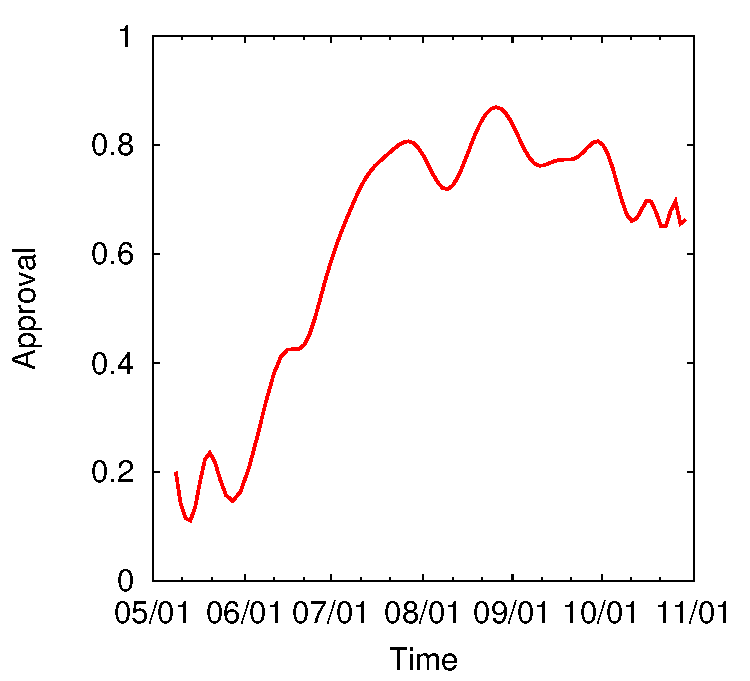
\includegraphics[width=2.1in,height=1.6in]{dilmaPositividade.pdf}}
\subfigure[MSE numbers as the stream evo\-lves.]{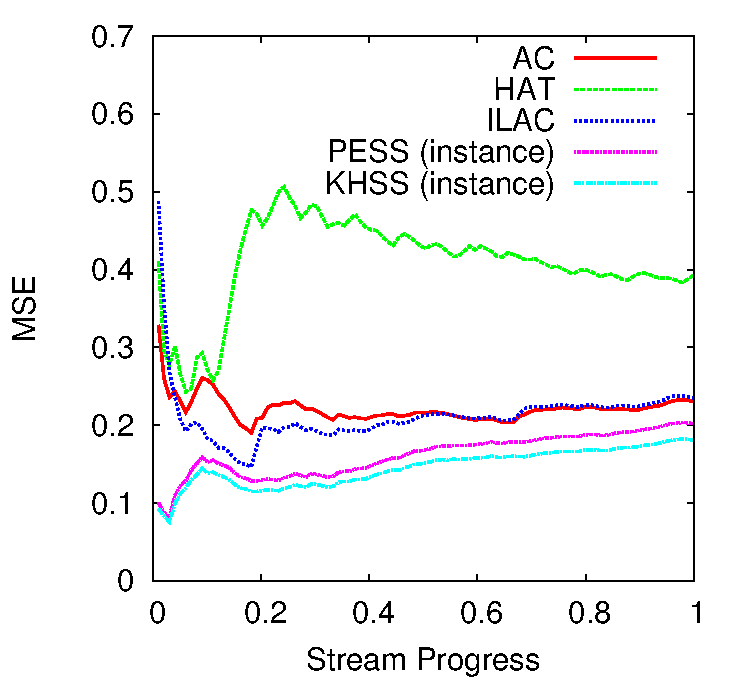
\includegraphics[width=2.1in,height=1.6in]{dilma_1_temporal_mse.pdf}}
\subfigure[X-Y scatter plot correlating the minimum similarity threshold $\alpha$ and labeling effort.]{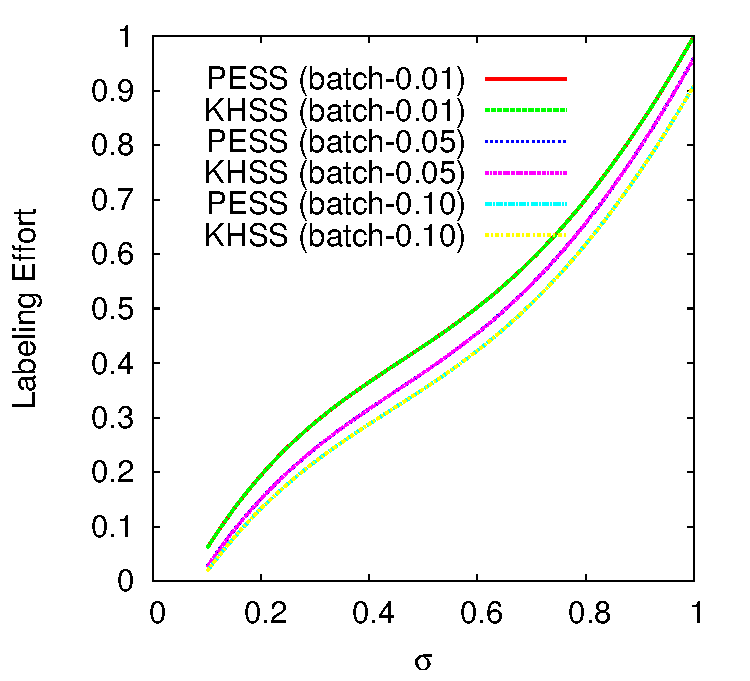
\includegraphics[width=2.1in,height=1.6in]{dilma_2_similaridade_rotulacoes.pdf}}
\subfigure[X-Y scatter plot correlating labeling effort and MSE numbers.]{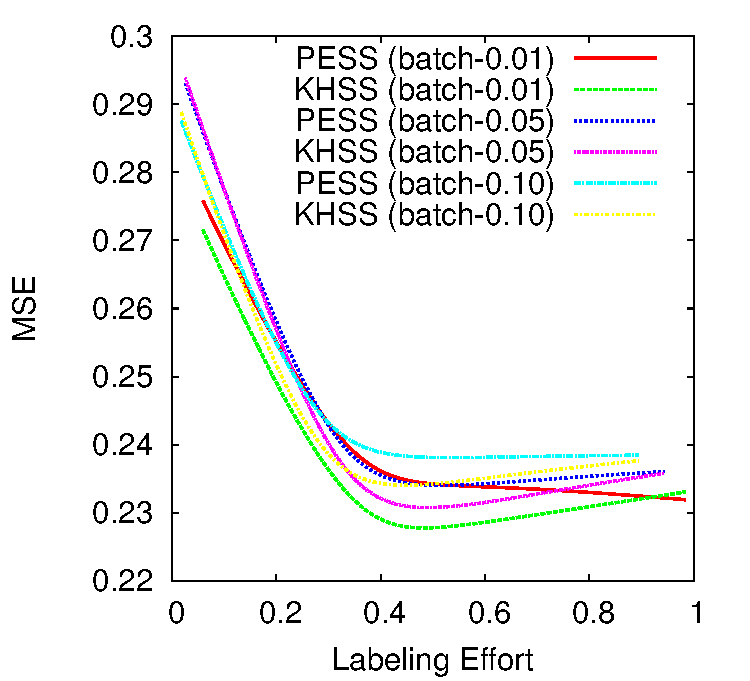
\includegraphics[width=2.1in,height=1.6in]{dilma_3_rmse-labelling.pdf}}
\subfigure[Size of the training sets as the stream evolves.]{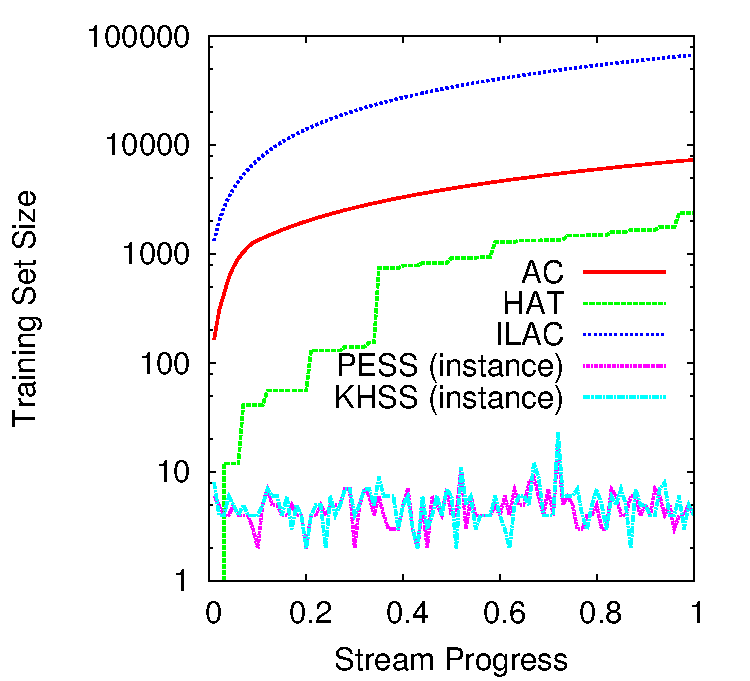
\includegraphics[width=2.1in,height=1.6in]{dilma_window.pdf}}
\subfigure[RAM-Hours as the stream evo\-lves.]{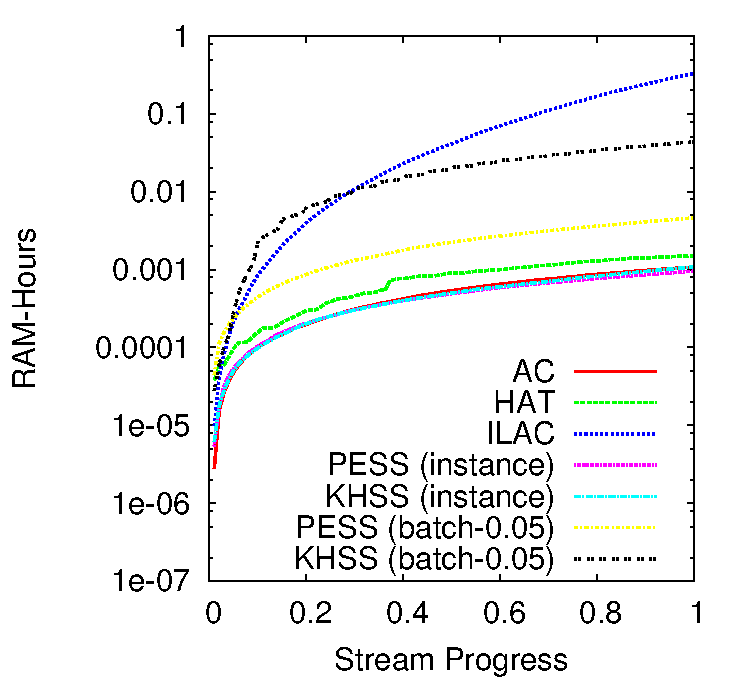
\includegraphics[width=2.1in,height=1.6in]{dilma_4.pdf}}
\caption{Brazilian Presidential Elections. Tweets are in Portuguese.}
\label{fig:dilma}
\end{figure*}

%  \subsection{Brazilian Presidential Elections}
%  
%  The presidential election campaigns were held from June to October 2010.
%  the candidate Dilma Rousseff launched a Twitter page during a public announcement, and she used Twitter as one of the main sources of information for her voters. The campaign attracted more than 500,000 followers and
%  as a result Dilma was the second most cited person on Twitter in 2010.
%  The election came to a second round vote, and Dilma Rousseff won the runoff with 56\% of the votes.
%  
%  \subsection*{Dilma Rousseff Election Campaign}
%  %\paragraph*{\bf{Dilma Rousseff Election Campaign}}
%  We collected 66,643 messages in Portuguese referencing Dilma Rousseff in Twitter during her campaign. We labeled these messages in order to track the population sentiment of approval during this period. As shown in Figure~\ref{fig:dilma} (a), approval varied significantly over the time due to several polemic statements and political attacks, and our goal is to score approval during her campaign.
%  %The dataset contains 62,089 distinct terms, and
%  %a message is posted every 50 seconds, on average.
%  
%  Figure~\ref{fig:dilma} (b) shows the results in terms of MSE obtained for the evaluation of the classifiers in this dataset. All classifiers evaluated in this experiment operate on an instance basis.
%  The x-axis represents different time steps (i.e., each message that
%  passes in the stream), while the y-axis shows the MSE so far.
%  As it can be seen, a better approximation is obtained using our proposed algorithms, namely PESS and KHSS.
%  %For this dataset, HAT was not effective, as its performance deteriorates as the stream evolves.
%  AC and ILAC were very competitive during all the campaign. Both PESS and KHSS algorithms started much better than the other competing algorithms, but slowly converges to the baseline numbers as the stream evolves.
%  
%  Figure~\ref{fig:dilma} (c) shows results concerning the proposed algorithms when operating in batch mode. The figure shows the number of messages that were labeled during the process as a function of $\delta$, the minimum similarity threshold discussed in Section 3.1. Basically, we calculate the Jaccard coefficient associated with each possible pair of messages in the batch, and if the coefficient is greater than $\delta$, the corresponding messages are merged into a new one. The process continues merging similar messages until no pair of messages are similar enough, and the process stops. At the end, only the merged messages are labeled. Clearly, higher values of $\delta$ implies that less messages are merged, and thus incurring more labeling effort. Further, as the figure shows, the dependence between labeling effort and $\delta$ tends to be linear.
%  %Also, both algorithms, PESS and KHSS, require the same amount of training resources during the process.
%  
%  By varying $\delta$, we also study the trade-off between labeling effort and MSE. As shown in Figure~\ref{fig:dilma} (d), MSE decreases if more labeling effort is spent during the process. Specifically, best results are achieved when about 40\% of the messages in the stream are labeled during the process. Although both PESS and KHSS require the same amount of training resources, KHSS provides slightly better MSE numbers. Furthermore, smaller batch sizes incur in less labeling effort for this dataset.
%  
%  We assume that HAT requires only the target message for updating its tree model, and thus we consider that the training set is composed only by the target message. The AC algorithm requires much more
%  messages within each training set. An abrupt decrease in the number of training messages is always observed after drifts.
%  %Although ILAC performs a data projection strategy that filters irrelevant messages at each time step, it is clear that the number of training messages still increases as the stream evolves.
%  The proposed PESS algorithm requires very small training sets, since the Pareto frontier at each time step is composed by few messages, but these messages are still able to make the classifier robust to drifts as the stream evolves. Further, despite being less stringent than PESS, the proposed KHSS algorithm also requires small training sets, as shown in Figure~\ref{fig:dilma} (e).
%  
%  Figure~\ref{fig:dilma} (f) shows RAM-Hours numbers for the algorithms. AC, as well as PESS (instance) and KHSS (instance), are clearly the best performers in terms of amount of computing resources required. Also, resources required during the process significantly increases when PESS and KHSS operate on batch mode, but still, ILAC is the worst performer.
%  
%  \subsection{TIME's Person of the Year}
%  
%  Every year, TIME magazine selects the person (or a group of persons) that
%  has mostly influenced during the year. The chosen person for 2010 was Mark Zuckerberg. The reader choice, however, was Julian Assange, with an overwhelming superiority of votes.
%  
%  \begin{figure*}[htp!]
%  \centering
%  \subfigure[MSE numbers as the stream evolves.]{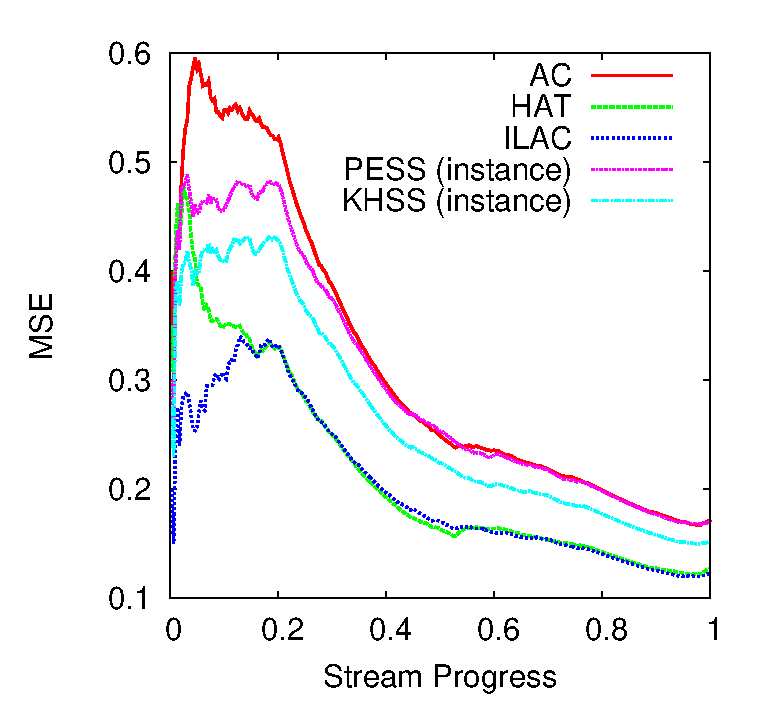
\includegraphics[width=2.2in,height=1.6in]{assange_1_temporal_mse.eps}}
%  \subfigure[X-Y scatter plot correlating labeling effort and MSE numbers.]{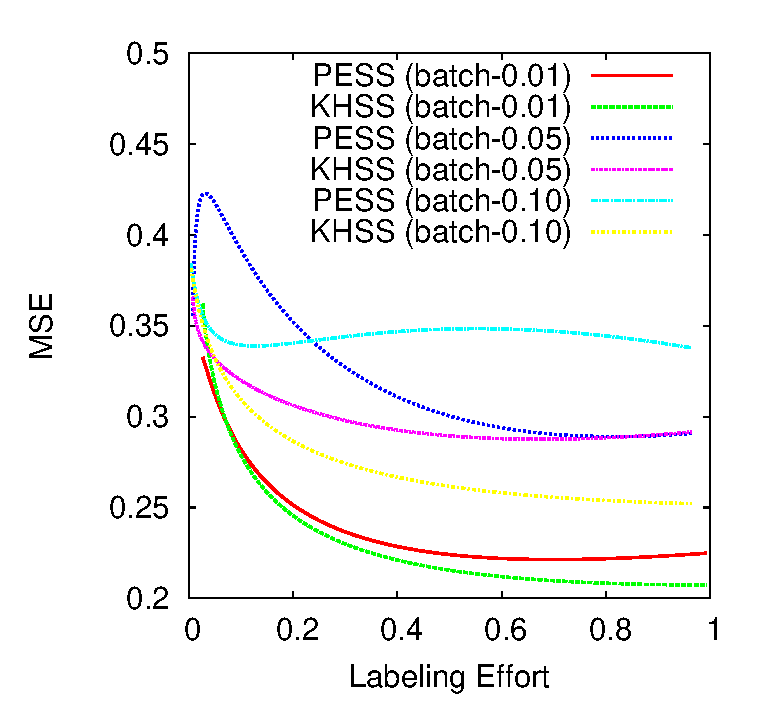
\includegraphics[width=2.2in,height=1.6in]{assange_3_rmse-labelling.eps}}
%  \subfigure[RAM-Hours as the stream evolves.]{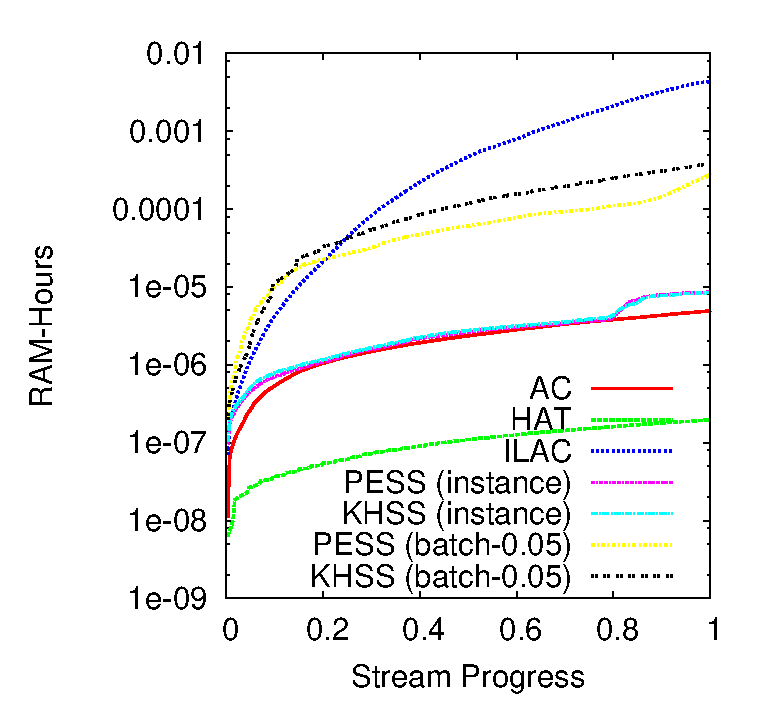
\includegraphics[width=2.2in,height=1.6in]{assange_4.1_ram-hours_instance_baseline.eps}}
%  \caption{Person of the Year. Tweets are in English.}
%  \label{fig:assange}
%  \end{figure*}
%  
%  \subsection*{Zuckerberg and Assange}
%  We collected 5,616 messages in English
%  referencing Julian Assange and Mark Zuckerberg from 1-15-2010 to 12-21-2010.
%  We labeled them in order to track diverse sentiments regarding the magazine's decision. Sentiments include (dis)approval, surprise (since the reader choice was pointing to Julian Assange),
%  and even fury.
%  The dataset contains 7,294 distinct terms, and
%  a message is posted every 45 seconds, on average.
%  
%  Figure~\ref{fig:assange} (a) shows the results in terms of MSE.
%  %The x-axis represents each message that
%  %passes in the stream, while the y-axis shows the MSE so far.
%  As it can be seen, a better approximation is obtained by HAT and ILAC.
%  For this dataset, AC was not effective in the first
%  time steps. At the end of the process, both PESS (instance) and KHSS (instance) algorithms achieved competitive numbers when compared against the best performers.
%  
%  Figure~\ref{fig:assange} (b) shows the trade-off between labeling effort and MSE. Again, MSE numbers decrease as more labeling effort is spent during the process. This trend is particularly evidenced for smaller batch sizes. Further, the KHSS algorithms shows a better trade-off between labeling effort and MSE.
%  Finally, Figure~\ref{fig:assange} (c)
%  shows RAM-Hours numbers for the evaluated algorithms. The AC algorithm, as well as PESS (instance) and KHSS (instance) are, again, extremely competitive in terms of amount of computing resources required. Further, the amount of resources required during the process significantly increases when PESS and KHSS operate on batch mode, but still, ILAC is the worst performer.
%  
%  \subsection{FIFA World Cup}
%  
%  The 2010 Soccer World Cup involved 32 teams. The Brazilian team was defeated by the Dutch team on 07-02-2010, after a controversial match. The Brazilian team scored first, but soon after the Dutch team scored twice and won the match. A specific player, Felipe Melo, had decisive participation (for better and worse) in all three goals. Specifically, Figure~\ref{fig:por} (a) shows how the appreciation for Felipe Melo varied during the match.
%  
%  \subsection*{The Brazilian Defeat}
%  %\paragraph*{\bf{The Brazilian Defeat}}
%  We collected 3,214 messages in Portuguese referencing Felipe Melo that were posted in Twitter as the match was happening.
%  We labeled them in order to track the
%  appreciation for the participation of Felipe Melo.
%  
%  Figure~\ref{fig:por} (b) shows the results in terms of MSE.% We assume that these messages expose the sentiment expressed by Brazilian Twitter users during the match.
%  %Again, the x-axis represents each message that
%  %passes in the stream, while the y-axis shows the MSE so far.
%  As it can be seen, the AC algorithm achieved the worst MSE numbers for this dataset. On the other hand, HAT, ILAC, as well as PESS (instance) and KHSS (instance) showed extremely competitive numbers. This is expected, since this dataset contains three sudden drifts (as shown in Figure~\ref{fig:por} (a)), and HAT, ILAC, PESS (instance) and KHSS (instance) were all able to ensure adaptiveness.
%  %either by updating the tree model or projecting the training set according to the target message, or by selecting messages by minimizing time and space distances.
%  For this dataset, memorability is not mandatory (as the sentiment distribution never returns to a pre-drift
%  distribution), and thus PESS (instance) and KHSS (instance) were not able to provide significant improvements, although being the best performers overall.
%  
%  Figure~\ref{fig:por} (c) shows a X-Y scatter plot correlating $\delta$ and labeling effort. The correlation is almost linear. The trade-off between labeling effort and MSE is shown in Figure~\ref{fig:por} (d). Clearly, MSE decreases with the effort spent to label messages.
%  Figure~\ref{fig:por} (e) shows the number of messages composing the training set at each time step.
%  As in previous cases, AC and ILAC require much more training resources than other competing algorithms. PESS (instance) as well as KHSS (instance) require much less training messages, again, showing that the selective sampling strategy is effective in producing small and effective sets at each time step.
%  
%  Finally, Figure~\ref{fig:por} (f)
%  shows RAM-Hours numbers. In this case, AC, as well as PESS (instance) and KHSS (instance), are clearly the best performers in terms of amount of computing resources required. Further, the amount of resources required during the process significantly increases when PESS and KHSS operate on batch mode, but still, as in other datasets, ILAC is the worst performer.
%  
%  \begin{figure*}[htp!]
%  \centering
%  \subfigure[Appreciation associated with Felipe Melo over the match.]{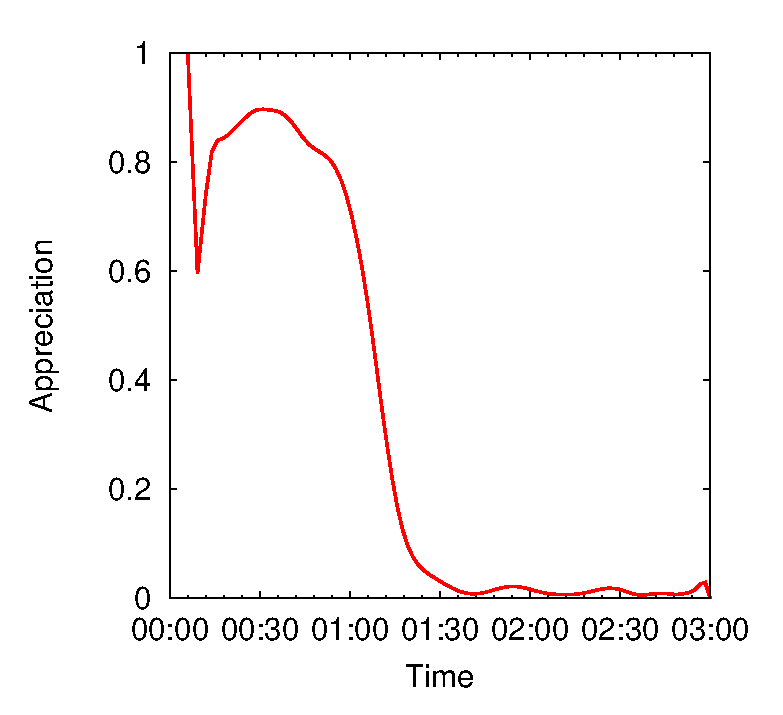
\includegraphics[width=2.2in,height=1.6in]{felipemeloPositividade.eps}}
%  \subfigure[MSE numbers as the stream evolves.]{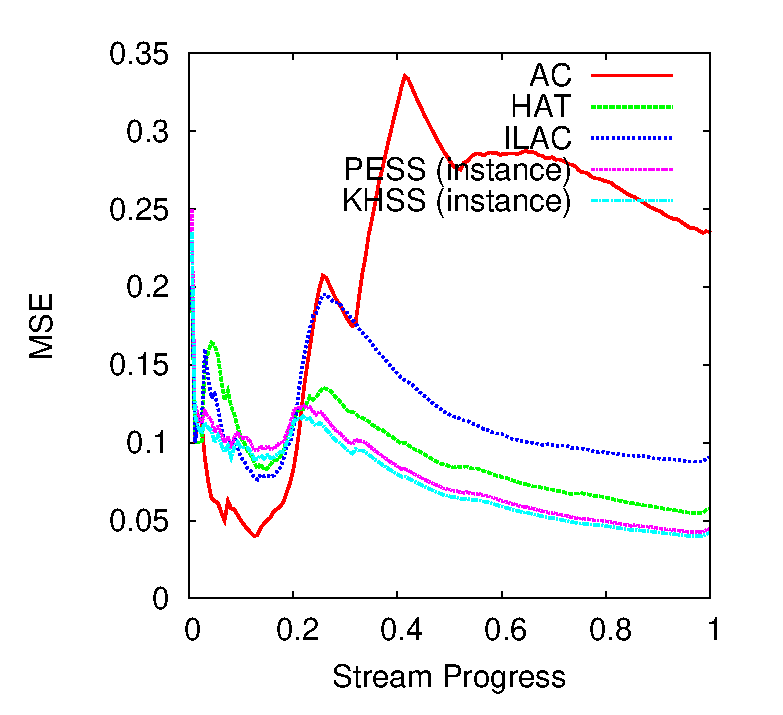
\includegraphics[width=2.2in,height=1.6in]{pt_1_temporal_mse.eps}}
%  \subfigure[X-Y scatter plot correlating the minimum similarity threshold $\delta$ and labeling effort.]{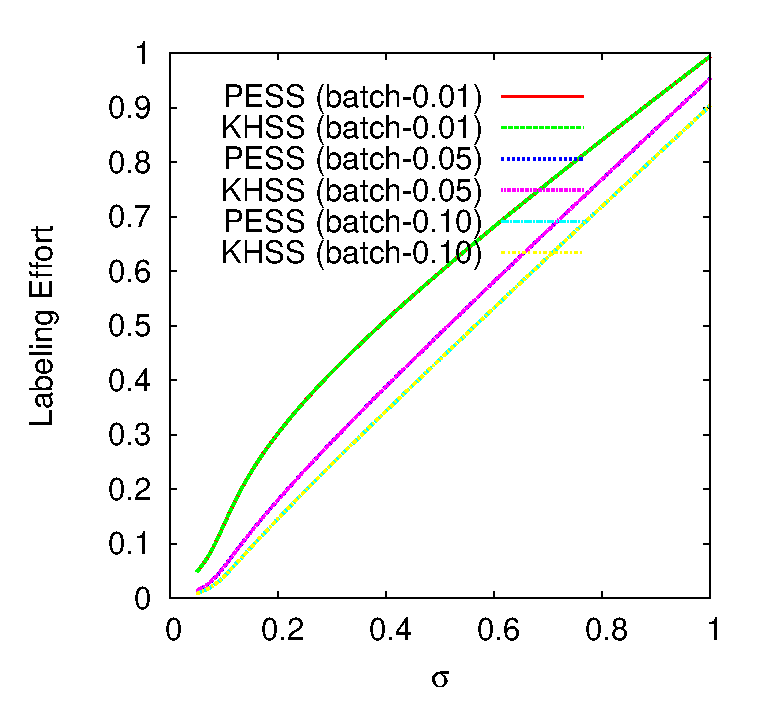
\includegraphics[width=2.2in,height=1.6in]{pt_2_similaridade_rotulacoes.eps}}
%  \subfigure[X-Y scatter plot correlating labeling effort and MSE numbers.]{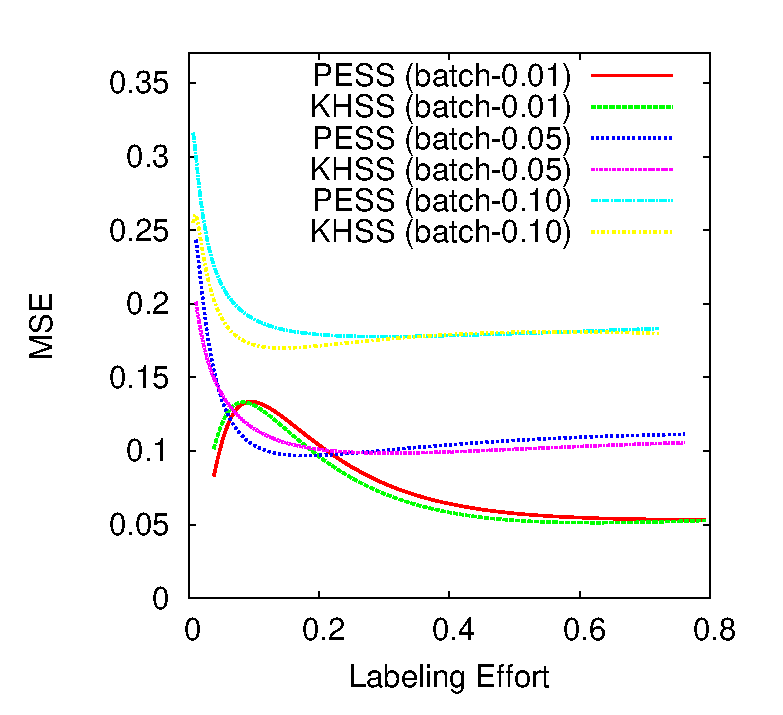
\includegraphics[width=2.2in,height=1.6in]{pt_3_rmse-labelling.eps}}
%  \subfigure[Size of the training sets as the stream evolves.]{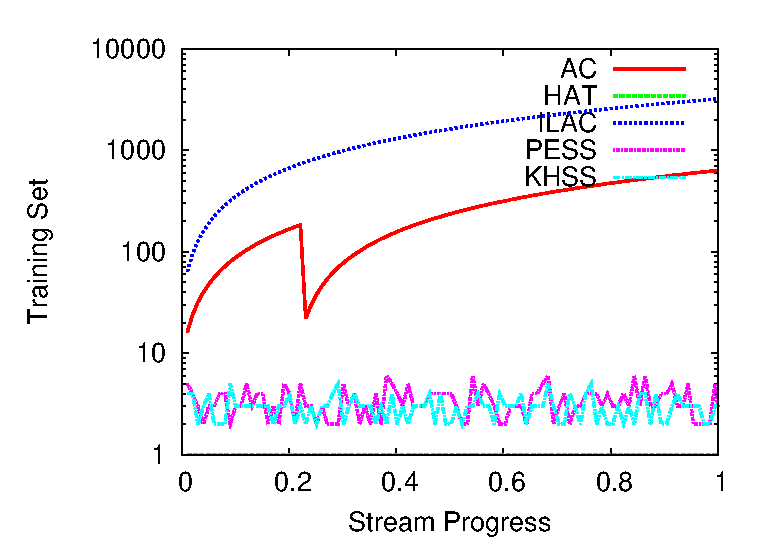
\includegraphics[width=2.2in,height=1.6in]{pt_window.eps}}
%  \subfigure[RAM-Hours as the stream evolves.]{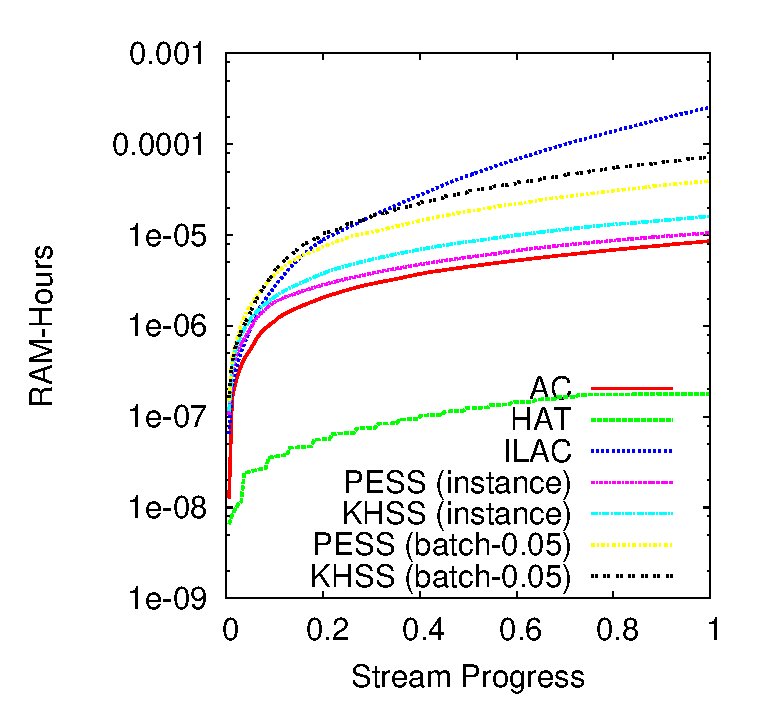
\includegraphics[width=2.2in,height=1.6in]{pt_4.1_ram-hours_instance_baseline.eps}}
%  \caption{The Brazilian Defeat. Tweets are in Portuguese.}
%  \label{fig:por}
%  \end{figure*}
%  
%  %The last set of experiments concerns the evaluation of the same event, but using the dataset composed of messages in English. By inspecting the dataset, we confirmed that most of the messages were posted by people in Europe, specially German, English and Dutch users. Such users showed conflicting or mixed sentiments as the match goes. As a consequence, drifts occur, but eventually the sentiment distribution returns to a pre-drift distribution, making memorability an important property while scoring sentiments in this dataset. This explains the reason why PESS (instance) and KHSS (instance) performed much better than the other competitors, as we can see in Figure~\ref{fig:eng} (a). Figure~\ref{fig:eng} (b) shows the trade-off between MSE and the amount of training resources needed during the process. Finally, Figure~\ref{fig:eng} (c) shows the amount of computing resources needed during the process.
%  
%  %\begin{figure*}[htb]
%  %\centering
%  %\subfigure[MSE numbers as the stream evolves.]{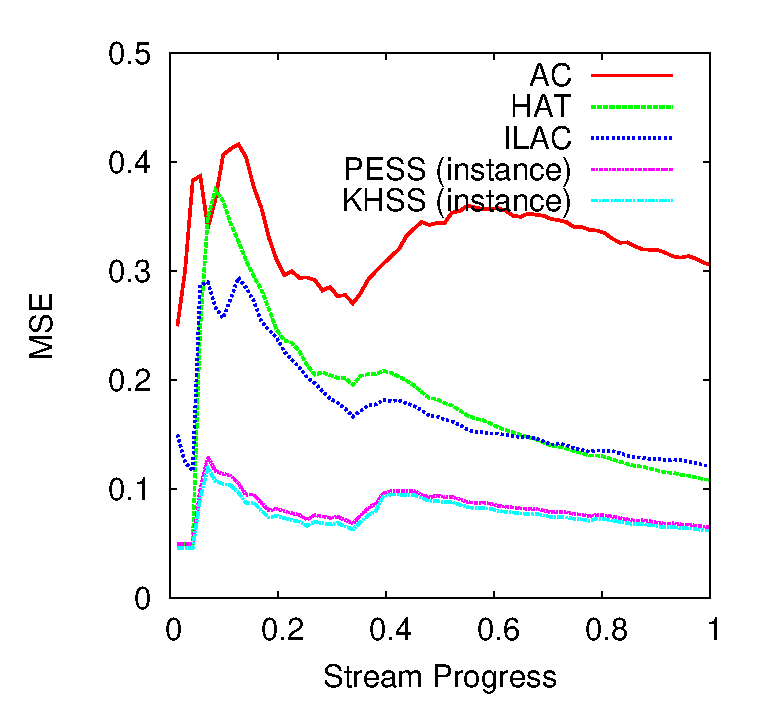
\includegraphics[width=2.1in,height=1.6in]{en_1_temporal_mse.eps}}
%  %\subfigure[X-Y scatter plot correlating labeling effort and MSE numbers.]{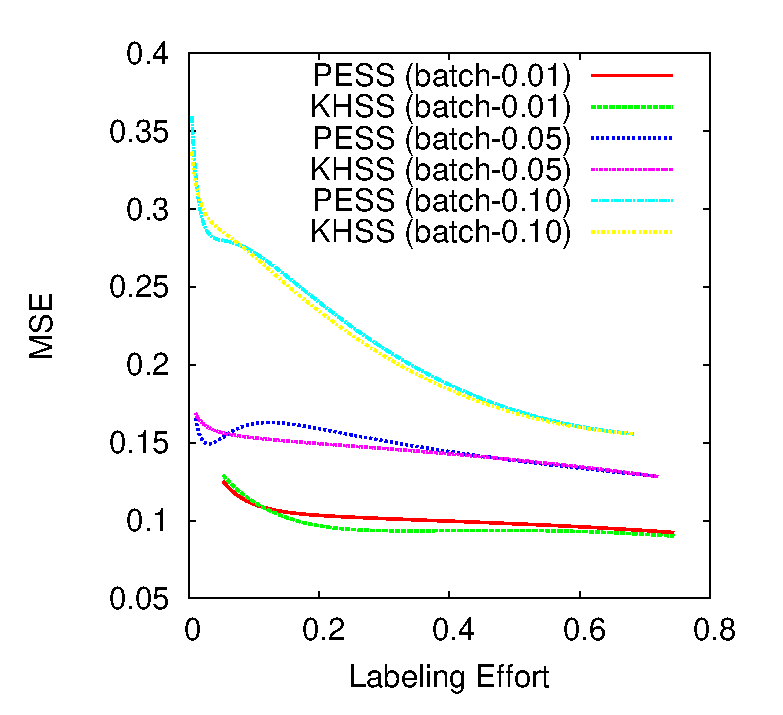
\includegraphics[width=2.1in,height=1.6in]{en_3_rmse-labelling.eps}}
%  %\subfigure[RAM-Hours as the stream evolves.]{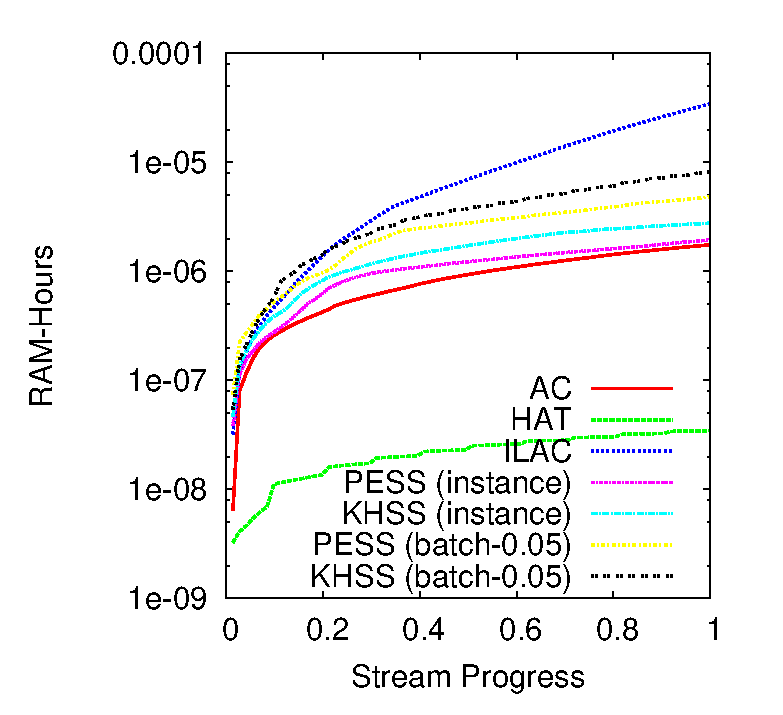
\includegraphics[width=2.1in,height=1.6in]{en_4.1_ram-hours_instance_baseline.eps}}
%  %\caption{The Brazilian Defeat. Tweets are in English.}
%  %\label{fig:eng}
%  %\end{figure*}

\section{Conclusions}

This paper focused on sentiment analysis on Twitter streams. We have introduced new algorithms for active training-set formation, which we denote as Pareto-Efficient Selective Sampling (PESS) and Kaldor-Hicks Selective Sample (KHSS). The proposed algorithms provide the resulting classifier with memorability and adaptiveness. We formalized the selective sampling process as a multi-objective optimization procedure, which finds a proper balance between adaptiveness and memorability.
Adaptiveness is assessed by computing the distance in time and space between the target message and the candidate ones. Also, candidate messages are randomly shuffled, thus providing memorability to the resulting classifier. The message utility space is composed by such dimensions, and we compute the Pareto Frontier in this space in order to pick up messages satisfying the Pareto improvement condition, finding a proper balance between adaptiveness and memorability. The Kaldor-Hicks criterion enables memorability to compensate adaptiveness, or vice-versa. A systematic evaluation involving recent events demonstrated the effectiveness of our algorithms.

As future work, we intend to extend our strategies for algorithms that do not depend on manual labeling.


\bibliographystyle{abbrv}
\bibliography{adriano,references}

\end{document}
